\documentclass[]{article}
\usepackage{lmodern}
\usepackage{amssymb,amsmath}
\usepackage{ifxetex,ifluatex}
\usepackage{fixltx2e} % provides \textsubscript
\ifnum 0\ifxetex 1\fi\ifluatex 1\fi=0 % if pdftex
  \usepackage[T1]{fontenc}
  \usepackage[utf8]{inputenc}
\else % if luatex or xelatex
  \ifxetex
    \usepackage{mathspec}
  \else
    \usepackage{fontspec}
  \fi
  \defaultfontfeatures{Ligatures=TeX,Scale=MatchLowercase}
\fi
% use upquote if available, for straight quotes in verbatim environments
\IfFileExists{upquote.sty}{\usepackage{upquote}}{}
% use microtype if available
\IfFileExists{microtype.sty}{%
\usepackage{microtype}
\UseMicrotypeSet[protrusion]{basicmath} % disable protrusion for tt fonts
}{}
\usepackage[unicode=true]{hyperref}
\hypersetup{
            pdfborder={0 0 0},
            breaklinks=true}
\urlstyle{same}  % don't use monospace font for urls
\usepackage{longtable,booktabs}
% Fix footnotes in tables (requires footnote package)
\IfFileExists{footnote.sty}{\usepackage{footnote}\makesavenoteenv{long table}}{}
\usepackage{graphicx,grffile}
\makeatletter
\def\maxwidth{\ifdim\Gin@nat@width>\linewidth\linewidth\else\Gin@nat@width\fi}
\def\maxheight{\ifdim\Gin@nat@height>\textheight\textheight\else\Gin@nat@height\fi}
\makeatother
% Scale images if necessary, so that they will not overflow the page
% margins by default, and it is still possible to overwrite the defaults
% using explicit options in \includegraphics[width, height, ...]{}
\setkeys{Gin}{width=\maxwidth,height=\maxheight,keepaspectratio}
\IfFileExists{parskip.sty}{%
\usepackage{parskip}
}{% else
\setlength{\parindent}{0pt}
\setlength{\parskip}{6pt plus 2pt minus 1pt}
}
\setlength{\emergencystretch}{3em}  % prevent overfull lines
\providecommand{\tightlist}{%
  \setlength{\itemsep}{0pt}\setlength{\parskip}{0pt}}
\setcounter{secnumdepth}{0}
% Redefines (sub)paragraphs to behave more like sections
\ifx\paragraph\undefined\else
\let\oldparagraph\paragraph
\renewcommand{\paragraph}[1]{\oldparagraph{#1}\mbox{}}
\fi
\ifx\subparagraph\undefined\else
\let\oldsubparagraph\subparagraph
\renewcommand{\subparagraph}[1]{\oldsubparagraph{#1}\mbox{}}
\fi

% set default figure placement to htbp
\makeatletter
\def\fps@figure{htbp}
\makeatother


\date{}

\begin{document}

\textbf{\emph{DISTURBI DI PERSONALITA':}}

\textbf{\emph{INTRODUZIONE:}}

\emph{``E' peggio essere malati nell'anima che nel corpo, perché i
malati nel corpo soffrono e basta, i malati nell'anima oltre a soffrire
edificano il loro male.''}

\begin{quote}
Plutarco
\end{quote}

Tutte le patologie psichiatriche (disturbi psicotici, d'ansia,
dell'umore, ecc.) assomigliano molto a delle patologie mediche: ad una
persona capita di ammalarsi di disturbo d'ansia, ad un'altra capita di
ammalarsi di schizofrenia. L'individuo esperisce dei sintomi e la lotta
contro la patologia è la lotta di questo individuo per la salute.

I disturbi di personalità sono molto diversi, si possono descrivere come
la quintessenza dei disturbi dell'anima. Questi malati oltre a soffrire,
citando Plutarco, edificano il loro male. È un disturbo tragico.

\textbf{\emph{PERSONALITA':}}

Per parlare di disturbo di personalità, occorre definire una personalità
normale, priva di un quadro patologico.

In condizioni normali secondo l'\textbf{\emph{organizzazione di
personalità}} di Kernberg, la personalità si caratterizza per:

\begin{itemize}
\item
  L'\textbf{Identità}, ovvero il \emph{senso di sé e della propria
  struttura interna}, che consente al paziente di organizzarsi, di
  pianificare, avere delle proprie risorse, dei valori e degli obiettivi
  di vita, sapendo anche come raggiungerli. Nelle forme patologiche di
  personalità, il senso di sé e degli altri appare frammentario, a volte
  estremo, altre volte instabile e superficiale, con marcata difficoltà
  nel comprendere gli altri e nel rispondere in modo adeguato, per cui
  nel paziente si può sviluppare un senso di vuoto, una disforia cronica
  con assenza di investimenti.
\item
  Il \textbf{Livello Predominante dei Meccanismi di Difesa}, cioè
  \emph{i modi di affrontare gli eventi stressanti sia esterni che
  interni}, per cui sono dei meccanismi adattativi, che ci permettono di
  andare avanti e di non suicidarci. Le risposte adattative possono in
  questo caso essere \textbf{\emph{mature}} (sono quelle fisiologiche,
  flessibili in base alla situazione, che ci consentono di interpretare
  la situazione stressante in maniera appropriata e reagire
  opportunamente per controllare lo stress senza distorcere la realtà
  interna o esterna), \textbf{\emph{nevrotiche}} (basate sulla
  \emph{rimozione}, cioè sul bandire dalla consapevolezza l'evento
  stressante, a notevole discapito della flessibilità della risposta,
  che spesso risulta quindi inadatta) o \textbf{\emph{primitive}}
  (basate sulla \emph{scissione}, cioè la compartimentazione delle
  condizioni spiacevoli, le quali risultano ``isolate'' le une dalle
  altre ed emergono in maniera alternata, mai assieme, dando una
  notevole instabilità tra le esperienze contradditorie).
\item
  L'\textbf{Esame della Realtà}, cioè la \emph{capacità di leggere ed
  interpretare i segnali sociali}, rispondendo in modo adeguato ai
  contatti interpersonali, e che viene meno nelle fasi più gravi dei
  disturbi di personalità, in genere in maniera del tutto inconsapevole
  per il soggetto, sebbene vada ricordato che \emph{una prolungata
  perdita dell'esame di realtà non è una caratteristica tipica dei
  disturbi di personalità}, sebbene nelle forme più gravi si possano
  comunque avere alterazioni transitorie, specie se legate a situazioni
  stressanti o all'uso di sostanze.
\item
  La \textbf{Qualità delle Relazioni Oggettuali}, cioè le relazioni
  interpersonali, che in una personalità normale si manifesta come la
  \emph{capacità di comprendere e tenere ai bisogni degli altri
  indipendentemente dai propri}, mentre nei disturbi di personalità
  predomina una visione delle relazioni improntata al soddisfacimento
  dei propri bisogni.
\end{itemize}

A queste quattro caratteristiche di base va poi aggiunta un ulteriore
elemento, che è il \textbf{funzionamento} \textbf{morale}, che
\emph{mette in relazione i valori ed i bisogni dell'individuo con quelli
della società} in cui il soggetto si trova a vivere: in condizioni
normali si ha una dedizione a valori ed ideali che si mantiene coerente
ma tuttavia flessibile, cioè sempre in relazione col senso di sé, mentre
nelle forme patologiche la flessibilità e l'integrazione nel sé viene
meno, ed il funzionamento morale può andare perso (come avviene ad
esempio nel DP antisociale) o risultare eccessivamente rigido ed
intransigente (come nei DP di Cluster C).

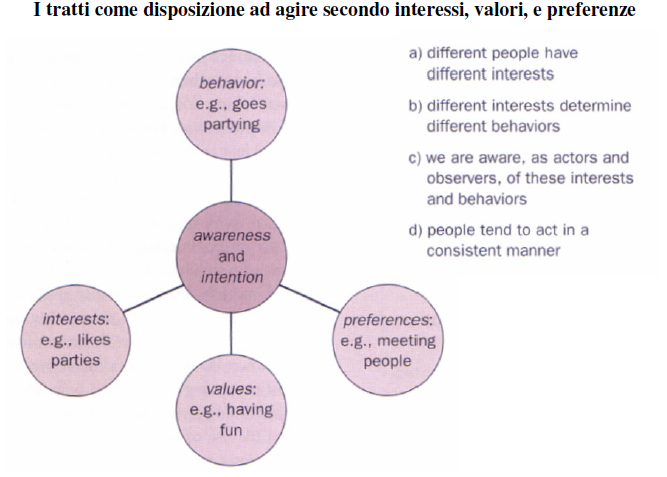
\includegraphics[width=3.89583in,height=3.34375in]{media/image1.png}Le
alterazioni dell'organizzazione della personalità sono quindi alla base
di tutte le varie forme di disturbo di personalità, ma bisogna tenere a
mente che la forma specifica di disturbo dipende dai
\textbf{\emph{tratti di personalità}} del soggetto, dove per tratti di
personalità si intendono dei \emph{modelli coerenti di comportamento,
emozioni e di stile cognitivo che dettano le differenze interindividuali
nel comportamento, rimanendo in genere stabili nel tempo o nei
contesti}. La differenza in tratti di personalità determina come noi ci
comportiamo in modo diverso l'uno all'altro, determina quindi la nostra
unicità.

Ad esempio, l'interesse potrebbe essere \emph{``mi piacciono le
feste'',} il valore \emph{``divertirmi}'', le preferenze
\emph{``incontrare gente nuova''}, il comportamento \emph{``vado
volentieri alle feste''}. Questo è un esempio di tratto di personalità.

Per questo motivo ci comportiamo in modo coerente, tant'è che è facile
anche per ciascuno di noi conoscendo i propri amici, prevedere il loro
comportamento. Se per esempio volessimo andare al cinema, sapremmo quale
amico sarebbe più disposto a venire. \emph{\emph{Questo ragionamento è
possibile perché conosciamo quali sono i suoi valori, i suoi interessi,
le sue preferenze e quindi ci è possibile prevedere il suo
comportamento. I tratti di personalità sono quelli che ci rendono
prevedibili e ci aiutano a stare insieme. }}

Ovviamente in tratti di personalità sono del tutto egosintonici, non
vengono avvertiti come problematici (nemmeno quando sono molto deviati
rispetto alla norma!) e a loro volta derivano da un'amalgama tra il
\textbf{\emph{temperamento}} (fattori genetici ereditabili che
influenzano la risposta all'ambiente) e l'\textbf{\emph{esperienza}},
cioè ciò che viene appreso nell'interazione con l'ambiente.

Il temperamento, più nello specifico, è la parte genetica dei tratti di
personalità. \textbf{È la tendenza innata a reagire ai vari stimoli
ambientali}. Innata non vuol dire non modificabile, però quando
nasciamo, già per il fatto di essere nati, abbiamo la nostra piccola,
unica disposizione (che già allora ci rende diversi e unici) a reagire
in un certo modo agli stimoli ambientali.

Da piccoli si può vedere relativamente poco, ma per esempio, c'è il
bambino che piange molto e c'è il bambino che si calma subito.

Il \textbf{\emph{temperamento}},ha delle \emph{caratteristiche
biologiche stabili ed ereditabili, geneticamente determinate}, che si
manifestano attraverso 4 \textbf{dimensioni temperamentali}, le quali
sono tra loro indipendenti:

\begin{enumerate}
\def\labelenumi{\arabic{enumi}.}
\item
  \textbf{Ricerca di stimoli forti e nuovi:}, potenzialmente piacevoli e
  gratificanti nell'ambiente. Rappresenta la nostra voglia di esplorare
  e di avere un reward, una gratificazione dagli stimoli dell'ambiente.
  Questa tendenza di chiama \textbf{ricerca della novità,} ed è
  responsabile, se eccessiva, di comportamenti di impulsività
  (\emph{``non mi basta mai''} -\textgreater{} abuso di sostanze) o,
  all'opposto, di comportamenti di eccessivo ritiro (``\emph{non mi
  interessa} `` -\textgreater{} non cerco niente di piacevole). alcuni
  soggetti hanno una forte tendenza alla ricerca di nuove situazioni,
  mentre altri non le ricercano affatto, risultando spesso noiosi agli
  occhi degli altri.
\item
  \textbf{Affettività negativa o sistema di inibizione comportamentale}.
  Rende conto della tendenza a reagire a stimoli nuovi e potenzialmente
  pericolosi. Esprime ``come vediamo l'ambiente'': è un ambiente denso
  di pericoli o no? Noi tutti variamo in questo. Avere troppa paura,
  quindi vedere troppi stimoli potenzialmente pericolosi nell'ambiente
  può portare a eccessiva inibizione. D'altro canto, avere troppa poca
  paura può dare ugualmente problemi, si rischia infatti di non imparare
  dagli stimoli negativi.
\item
  \textbf{Capacità di risuonare in base ai rinforzi sociali}: è la
  nostra capacità di legarci agli altri, la capacità di attaccamento.
  Quanto siamo intaccati da quello che gli altri pensano/dicono di noi e
  da quanto ci stanno vicini.\\
  Se pensiamo all'esclusione interpersonale, è studiatissima in
  psicologia sociale perché noi esseri umani siamo esseri sociali, e
  quindi dobbiamo stare insieme, infatti abbiamo un sistema nel cervello
  chiamato \textbf{sistema per il riconoscimento
  dell'ostracismo}\emph{.} Questo sistema si attiva quando il soggetto
  viene isolato da un gruppo di persone e attiva le stesse aree del
  dolore fisico. Quindi essere ostracizzati è dolorosissimo.
\end{enumerate}

\begin{quote}
È importante soffrire se gli altri ci abbandonano perché è un campanello
d'allarme. Il dolore sociale ci allerta del pericolo dell'esclusione
sociale, ci dice che c'è qualcosa che non sta andando.

Il segnale ha inizio nella corteccia anteriore del cingolo, prosegue poi
verso la corteccia dorsolaterale prefrontale, che fa modificare il
comportamento in un senso teso a fare riaccettare il soggetto agli
altri.\\
Il problema è che anche in questo caso, essendo una dimensione del
temperamento, è meglio non averne né troppo, né troppo poco. Chi ne ha
troppo poco potrebbe ricordare il primo paziente con Cluster A: infatti
predispone a un isolamento sociale, a una mancanza di empatia. D'altra
parte, averne tanto è ugualmente negativo, in gergo psicologico è
definito \emph{sentimentalismo}. Essere troppo sentimentali vuol dire
essere troppo dipendenti dal giudizio altrui, e potrebbe portare a
compiere azioni spiacevoli per noi stessi pur di tenerci legato chi ci
vuole escludere.

Quindi in alcuni casi si può avere un'ipersensibilità al rifiuto, mentre
in altri casi si ha una totale indifferenza alle lodi o al biasimo degli
altri.
\end{quote}

\begin{enumerate}
\def\labelenumi{\arabic{enumi}.}
\item
  Mentre le prime tre dimensioni sono abbastanza automatiche poiché
  conseguono a uno stimolo, la quarta dimensione, chiamata
  \textbf{capacità di autoregolazione}, serve per regolare tutte queste
  tendenze, serve per dire, per esempio: \emph{``Ho un obiettivo:
  quindi, anche se volessi usare cocaina tutti i giorni perché sono un
  impulsivo, questo interferirebbe col mio obiettivo, che è fare
  medicina''.}
\end{enumerate}

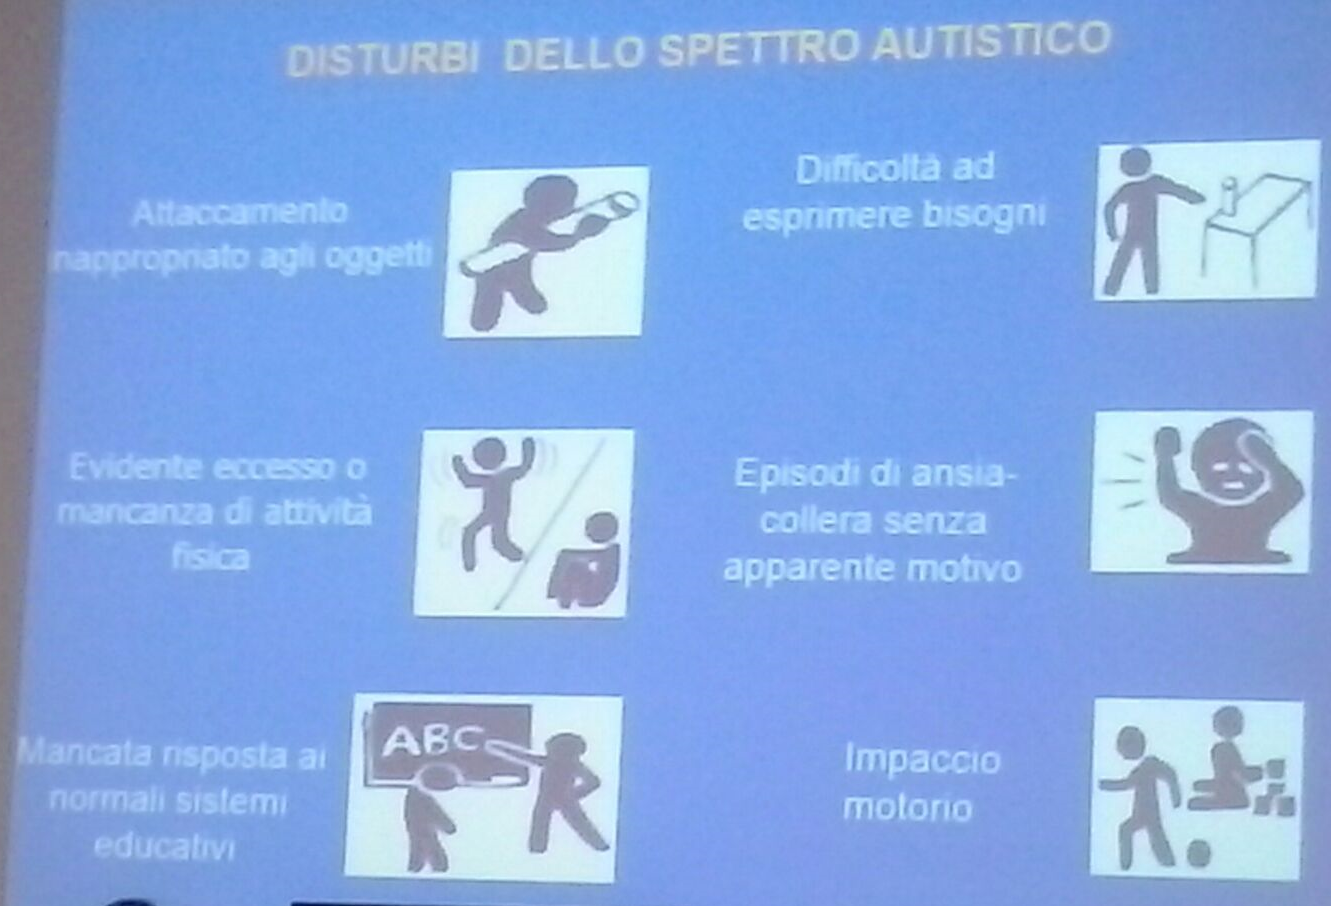
\includegraphics[width=3.50000in,height=2.53194in]{media/image2.png}Ogni
tratto temperamentale si distribuisce normalmente nella popolazione
generale, quindi tutti abbiamo tutti i tratti. La maggioranza delle
osservazioni saranno quindi nell'area centrale o appena laterale. La
maggior parte della popolazione avrà punteggi intermedi, che non
dovrebbero dare grossi problemi. Quando i tratti temperamentali sono
estremi, quindi o troppo alti o troppo bassi, ecco che si costruiscono
anche le prime basi dei problemi.

Il temperamento non è tutta la personalità. Si dice che, a partire dai
tratti temperamentali, io nasco, faccio le mie cose, in parte
selezionate dai miei tratti temperamentali, perché se io sono molto
pauroso tenderò a fare le cose con più cautela.

Le nostre esperienze ed anche un certo apprendimento forgiano i tratti
temperamentali fino a costituire la personalità a tutto tondo.

La personalità si articola in più parti, che riguardano tutte le
modalità di comportamento apprese a partire dai tratti temperamentali e
dalle esperienze di vita. È il modo in cui vediamo il mondo e ci
rapportiamo ad esso. Dunque la definizione di personalità è operativa:
cosa faccio, cosa voglio, quello che si vede fuori di me\ldots{}ecc.

\textbf{\emph{DEFINIZIONE:}}

Quando si fa il salto PERSONALITA' NORMALE DISTURBO DI PERSONALITA'?

Se i tratti di personalità diventano rigidi, intensi, si amplificano e
perdono flessibilità, si parla di disturbi di personalità.

Disturbo di personalità: \textbf{Fallimento che coinvolge 3 aree di
funzionamento dell'individuo, distinte, ma tra loro collegate:
\emph{sistema del Sé}, \emph{relazioni familiari o di parentela},
\emph{relazioni sociali o di gruppo}.}

\begin{itemize}
\item
  \emph{\textbf{Sistema del Sé}}: è l'idea che io ho di me, quello che
  voglio da me e dalla vita, i miei obiettivi e i miei valori.
\item
  \emph{\textbf{Relazioni familiari}}: come sto con i miei familiari,
  che possono essere: padre, madre, marito/moglie, figli.
\item
  \emph{\textbf{Relazioni sociali}}.
\end{itemize}

Cosa c'è nella vita di una persona, oltre a questi tre ambiti, che non
viene intaccato?

Nella vita di una persona normale non avanza nulla, non esista niente al
di fuori di queste tre aree.

\textbf{Il disturbo di personalità è un fallimento dell'individuo nella
sua interezza.}

Chiaramente questa è una definizione, non significa che tutti i soggetti
affetti da DP sono ugualmente deteriorati in tutte queste aree.

Secondo la definizione del OMS, il disturbo di personalità è un
\textbf{\emph{grave disturbo nel carattere e nelle tendenze
comportamentali dell'individuo, che in genere coinvolge diverse aree
della personalità ed è pressoché invariabilmente associato a gravi
deficit personali o sociali}}. Secondo la definizione di Livesley del
1998, inoltre, il disturbo di personalità può essere visto come ``
\emph{un fallimento che coinvolge tre aree funzionali dell'individuo,
distinte ma correlate: il sistema del Sé, le relazioni familiari e di
parentela e le relazioni sociali o di gruppo}''.

Per meglio definire le caratteristiche di questi disturbi si ricorre ai
criteri del DSM-IV TR, che devono essere presenti per poter porre
diagnosi corretta di disturbo di personalità:

\begin{enumerate}
\def\labelenumi{\arabic{enumi}.}
\item
  Dev'essere presente un \textbf{modello abituale di esperienza
  interiore e di comportamento che devia marcatamente rispetto alle
  aspettative culturali dell'individuo}, manifestandosi in 2 o più delle
  seguenti aree:
\end{enumerate}

\begin{itemize}
\item
  \textbf{\emph{Cognitività}} (cioè il modo di percepire ed interpretare
  se stessi, gli altri e gli avvenimenti che ci circondano); Sono cose
  che noi facciamo in automatico. Nei pazienti con DP qui c'è una
  distorsione: percepiscono se stessi, gli altri e gli avvenimenti in
  modo distorto.
\item
  \textbf{\emph{Affettività}} (cioè la varietà, l'intensità e
  l'adeguatezza della risposta emotiva); :.
\item
  \textbf{\emph{Funzionamento Interpersonale}}; ovvero realtà esterna,
  come io funziono con gli altri
\item
  \textbf{\emph{Controllo degli Impulsi}}. comportamento + realtà
  esterna.
\end{itemize}

\begin{enumerate}
\def\labelenumi{\arabic{enumi}.}
\item
  Tale modello abituale risulta \textbf{inflessibile e pervasivo} in
  un'ampia varietà di situazioni personali e sociali. Avere una
  difficoltà nel controllo degli impulsi (non è il singolo impeto d'ira
  che porta a fare magri un gesto sconsiderato). È un comportamento
  ricorrente.
\item
  Il modello abituale determINa un \textbf{disagio clinicamente
  significativo e compromissione del funzionamento} sociale, lavorativo
  e di altre aree inportanti.
\item
  Il modello si presenta \textbf{stabile e di lunga durata}, e l'esordio
  può essere fatto risalire almeno all'adolescenza o alla prima età
  adulta. Non si fa formalmente diagnosi prima dei 18-20 anni perché la
  personalità è ancora in evoluzione per tutta l'adolescenza e
  probabilmente per prima parte dell'età adulta, però in realtà
  clinicamente gli antecedenti dei DP dell'età adulta si vedono anche
  negli adolescenti.
\item
  Il modello abituale \textbf{non risulta meglio giustificato da una
  pregressa malattia psichiatrica o dall'assunzione di sostanze} ad
  azione psicotropa.
\end{enumerate}

Da questi criteri si può quindi concludere che i pazienti con disturbo
di personalità sono soggetti che si caratterizzano per
un'\textbf{\emph{incapacità stabile e pervasiva di amare e di
lavorare}}.

\emph{Amare} è da intendere in senso lato: avere relazioni reciproche
soddisfacenti (anche di amicizia o buona colleganza).

\emph{Lavorare} significa avere un obiettivo, applicarsi per
quell'obiettivo e farlo funzionare nella vita di tutti i giorni.

Per adottare una vecchia definizione di Schneider, si può dire che i
pazienti con disturbi della personalità sono ``\emph{pazienti che, per
il loro modo di essere fatti, soffrono o fanno soffrire gli altri}''.

\textbf{\emph{DIAGNOSI:}}

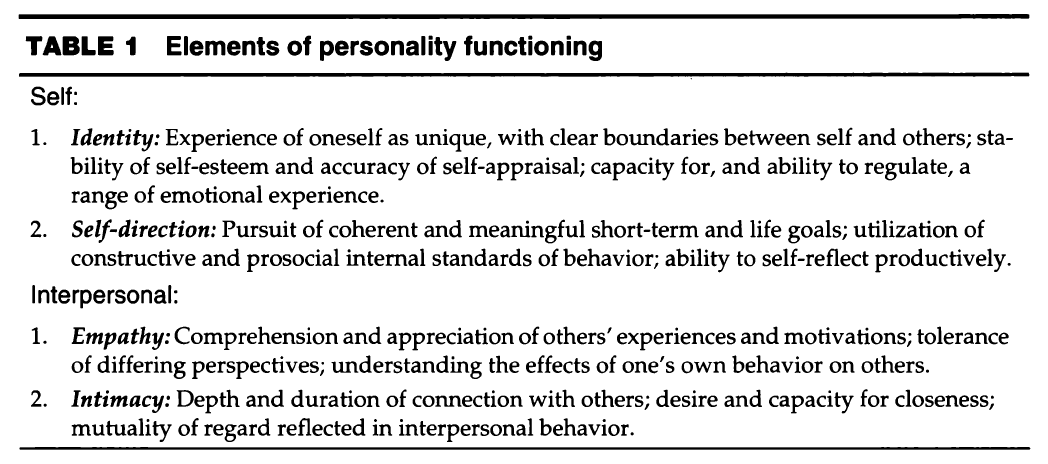
\includegraphics[width=4.76458in,height=2.72014in]{media/image3.png}Questi
sono gli elementi da valutare per la diagnosi generale di DP. Se non c'è
un disfunzionamento in queste 4 aree, non c'è un disturbo di
personalità.

\begin{itemize}
\item
  \emph{Disfunzionamento nel sé:}
\end{itemize}

\begin{enumerate}
\def\labelenumi{\arabic{enumi}.}
\item
  \emph{Concetto di identità}: esperienza di me stesso come unico,
  chiari confini tra sé e gli altri, stabilità dell'autostima,
  accuratezza della valutazione di sé, capacità di regolare un intero
  range di esperienza emotiva.
\item
  \emph{Autodirezionalità}: capacità di cercare e perseguire obiettivi
  di vita coerenti e con significato sia a lungo che a breve termine,
  valori morali e di senso etico.
\end{enumerate}

\begin{itemize}
\item
  \emph{Disfunzionamento delle realtà interpersonali}
\end{itemize}

\begin{enumerate}
\def\labelenumi{\arabic{enumi}.}
\item
  \emph{Disfunzione nell'empatia}: persone che in vario modo non
  riescono a comprendere ed apprezzare le motivazioni degli altri e a
  capire l`effetto del proprio comportamento sugli altri.
\item
  \emph{Disturbo dell'intimità.}
\end{enumerate}

\textbf{\emph{EPIDEMIOLOGIA E SFIDE DEI DP:}}

I disturbi di personalità sono patologie psichiatriche relativamente
comuni nella popolazione generale, in cui si stima abbiano una
\emph{prevalenza del 10-15\%}, e purtroppo sono disturbi che tendono
frequentemente ad associarsi ad altre condizioni psichiatriche, di cui
complicano la diagnosi, il decorso e soprattutto la terapia: tra queste
vanno ricordate l'abuso di alcol e sostanze, nonché gli episodi
depressivi ed i disturbi d'ansia, ma non bisogna dimenticare che questi
pazienti avranno comunque difficoltà relazionali, problemi abitativi e
disoccupazione frequente, ed hanno un maggior rischio di morte per
suicidio o per altre cause. All'interno dei pattern psichiatrici,
inoltre, come già accennato, la prevalenza di questi disturbi tende ad
essere molto più elevata, arrivando a soglie anche del 50-70\%, proprio
perché raramente questi disturbi si presentano in forma isolata.

Per definizione, il paziente con disturbo di personalità è ``\emph{il
paziente che non piace agli psichiatri}'', per il semplice fatto che
quando giungono all'attenzione medica (spesso costretti dagli altri, in
quanto loro si ritengono generalmente normali) hanno una
\emph{presentazione clinica urgente e caotica}, sono difficilmente
trattabili, e presentano una \emph{combinazione di diversi quadri}, che
vanno dall'autolesionismo all'abuso di sostanze e a problemi
interpersonali di tutti i tipi. Inoltre, ciò che risulta veramente
complesso con questi pazienti è la \emph{terapia}, poiché sono soggetti
con una \emph{bassissima compliance}, e tendono ad abbandonare il
trattamento anche in pochi giorni (il cosiddetto fenomeno delle
``\emph{revolving doors}''), salvo ripresentarsi dopo poco tempo al
pronto soccorso per fenomeni di autolesionismo o attacchi d'ansia. Per
tali motivi, i pazienti con disturbi di personalità \emph{inducono un
senso di inadeguatezza ed incertezza nello psichiatra}, poiché non sono
per niente facili da gestire e sono del tutto restii ad instaurare
un'alleanza terapeutica col medico.

\textbf{\emph{CLASSIFICAZIONE DEI DISTURBI DI PERSONALITÀ:}}

I disturbi di personalità vengono tipicamente suddivisi in tre gruppi
principali, detti ``\textbf{\emph{clusters}}'', indicati con le lettere
dell'alfabeto \textbf{A}, \textbf{B} e \textbf{C}.

Questo significa che comunque questi pazienti vedono soddisfatti tutti
quei criteri generali di cui abbiamo parlato finora, ma cambia per ogni
gruppo il modo in cui queste difficoltà vengono manifestate.

\begin{longtable}[]{@{}lll@{}}
\toprule
\textbf{\emph{Cluster A}} & \textbf{\emph{Cluster B}} &
\textbf{\emph{Cluster C}}\tabularnewline
\midrule
\endhead
\begin{minipage}[t]{0.32\columnwidth}\raggedright\strut
\begin{itemize}
\item
  \emph{DP Schizotipico}
\item
  \emph{DP Schizoide}
\item
  \emph{DP Paranoide}
\end{itemize}\strut
\end{minipage} & \begin{minipage}[t]{0.32\columnwidth}\raggedright\strut
\begin{itemize}
\item
  \emph{DP Antisociale}
\item
  \emph{DP Narcisistico}
\item
  \emph{DP Istrionico}
\item
  \emph{DP Borderline}
\end{itemize}\strut
\end{minipage} & \begin{minipage}[t]{0.32\columnwidth}\raggedright\strut
\begin{itemize}
\item
  \emph{DP Evitante}
\item
  \emph{DP Dipendente}
\item
  \emph{DP Ossessivo-Compulsivo}
\end{itemize}\strut
\end{minipage}\tabularnewline
\bottomrule
\end{longtable}

\textbf{\emph{Cluster A: ``eccentrico''}}

Il paziente del cluster A i caratterizza per la presenza di pensieri e
comportamenti bizzarri o inusuali, e anche per un'incapacità o
disinteresse nello stabilire relazioni soddisfacenti.

Riferendoci ai criteri generali, possiamo affermare che questi pazienti
hanno difficoltà nella cognitività (mondo interno): i pensieri sono
bizzarri e inusuali. A livello interpersonale (mondo esterno) hanno un
disinteresse a stabilire relazioni soddisfacenti.

\emph{Caso clinico: Paziente maschio, inviato dal medico di medicina
generale (MMG) ai servizi, dopo la morte del padre con cui viveva.}

\emph{Il MMG nel raccontare il caso ai colleghi dei servizi psichiatrici
racconta quello che sa della famiglia e quello che il pz nel corso del
tempo gli ha detto:}

\emph{Il pz descriveva il padre come distante, e in anamnesi aveva avuto
un `esaurimento nervoso' in gioventù e, secondo il paziente, il padre
`sentiva le voci' {[}probabilmente aveva un disturbo dello spettro
schizofrenico{]}. Spesso il pz quando andava a trovare il medico curante
si lamentava con lui di come il SSN avesse `abbandonato' il padre, ma
negava di avere egli stesso problemi di salute. Era però da sempre
affascinato dall'occultismo, e pensava continuamente all'eutanasia,
specie dopo la morte del padre.}

\emph{Anamnesi fisiologica: Era stato un bambino timido e un adolescente
solitario, senza mai aver avuto contatti al di fuori del nucleo
familiare. Aveva lavorato solo a tratti, per brevi periodi e in
situazioni solitarie, cioè lavori in cui non ci fossero colleghi (es
magazziniere). Era stato coinvolto in qualche `zuffa' in strada, ma non
aveva mai riportato condanne. Non aveva mai avuto esperienze sessuali né
sentimentali. Ora viveva solo con la madre anziana.}

Analizzando la breve storia in base ai criteri generali rileviamo:

\begin{itemize}
\item
  Mondo interno: uniche preoccupazioni sono cose un po' bizzarre
  (pensare solo all'eutanasia) -\textgreater{} alterazioni nella
  cognitività.\\
  zuffe in strada -\textgreater{} difficoltà nel controllo degli impulsi
\end{itemize}

\begin{itemize}
\item
  Realtà esterna: mai avuto rapporti di amicizia/ sentimentali
  -\textgreater{} deficit nelle relazioni interpersonali.
\end{itemize}

\emph{Ai colloqui psichiatrico si presenta scarsamente accessibile (non
parla), appare assorto nei propri pensieri; trova difficile rispondere
alle domande dello psichiatra, anche alle più banali. Risponde quasi a
monosillabi e in modo molto minimizzante. Tuttavia non vi sono segni di
disturbo dell'umore o psicosi. La madre riferisce che il pz come sua
unica attività (pz disoccupato) passa il tempo su internet, a fare
ricerche sull'eutanasia, e che ciò `non è sano'.}

Questo è un esempio di disturbo schizotipico di personalità. Può
preludere alla schizofrenia, tra tutti i disturbi è un po' diverso,
perché fa parte del cosiddetto spettro schizofrenico, costituisce la
vulnerabilità genetica alla schizofrenia: infatti è più frequente nei
familiari di I grado di pazienti con schizofrenia, e viceversa. Non ci
sono franchi deliri, non ci sono franche allucinazioni, ma c'è comunque
il distacco dagli altri.

\emph{In questo caso è necessaria una valutazione delle abilità sociali
e lavorative (dal momento che è incline a scoppi di rabbia, se gli viene
richiesto di essere più socievole) e del rischio per sé ed altri (es: vs
la madre, per via dei pensieri circa la eutanasia).}

\textbf{\emph{Cluster B: ``drammatico''}}

Sono fra i pazienti più difficili per gli psichiatri, \emph{``the
patients psychiatrists dislike''.}

Si caratterizzano per la presenza di comportamenti impulsivi, teatrali,
esagerati e instabili. L'instabilità è la quintessenza di questi
disturbi, riguarda sia mondo esterno che mondo interno.

Caso clinico: \emph{Ragazza di 22 anni, già nota ai servizi
psichiatrici; disoccupata. Ricoverata in servizio psichiatrico di
diagnosi e cura (SPDC) un sabato notte (in urgenza), dopo accesso al PS
per essersi tagliata i polsi a seguito di una lite con l'ex fidanzato.
Questa è solo l'ultima di una serie di relazioni violente con gli
uomini, tutte durate non più di alcuni mesi. La pz è già rimasta incinta
5 volte, ma solo 2 gravidanze erano andate a termine, e i 2 i figli
erano stati entrambi affidati ai servizi sociali alla nascita.}

\emph{\\
}Analizzando la situazione in base ai criteri generali dei DP si
riconosce facilmente il disfunzionamento interpersonale. La definizione
generale dice: ``incapacità di amare e lavorare'', non ci dice come. Nel
pz di prima c'era disinteresse e distacco, in questo invece sembra
esserci ipercoinvolgimento.

Emerge altresì il quadro tipico di inflessibilità e pervasività del
disturbo. Non si può dire che la pz sia stata sfortunata: ha trovato un
uomo violento e poi si è messa con uno bravo, ha continuato ad avere
relazioni violente con gli uomini. Allo stesso modo il pz del caso
precedente non si era isolato in un periodo della sua vita, era sempre
stato isolato\emph{. Il pattern è inflessibile, pervasivo in una varietà
di contesti sociali e interpersonali.}

Da ricordare anche come nella popolazione generale questi soggetti
vadano incontro a tutta una serie di problemi (disoccupazione, problemi
relazionali, ecc.), nella fattispecie l'allontanamento, appena dopo la
nascita, dei due figli.

\emph{La pz è figlia di una relazione di breve durata tra il padre e la
madre, che in seguito ebbe molti partners, qualcuno dei quali abusava
sessualmente della pz. Descritta come intelligente alle elementari,
inizia però presto a marinare la scuola e già alle medie viene sospesa
per aggressività sia verbale che fisica verso un insegnante e per uso di
droghe `leggere'. Dopo aver lasciato la scuola (alle medie), inizia ad
usare eroina e a prostituirsi per procurarsela. }

Da notare il disfunzionamento interpersonale che si manifesta con
l'aggressività. È chiaro inoltre che il compito di una bambina di 12
anni dovrebbe essere quello di andare a scuola, avere degli amici e
crescere, non di marinare la scuola, farsi sospendere e usare droghe
``leggere''. \emph{Il modello quindi devia rispetto alle aspettative
della cultura dell'individuo, c'è un fallimento nelle aree del sé.}

Ad un'analisi più attenta si notano delle similitudini tra la storia
della pz e quella della madre. Non è un evento casuale, sicuramente
hanno un ruolo la base genetica e un ``apprendimento'' del vissuto
materno. L'abuso sessuale costituisce poi un'aggravante ulteriore in
questa storia, soprattutto considerando il tipo di uomini ugualmente
violenti che poi ricerca la pz. La devianza si nota dal fatto che a
seguito di un'esperienza negativa si perpetui la ricerca di relazioni
abusanti con gli uomini.

Plutarco diceva che sono persone che edificano il loro male: c'è
qualcosa in lei che le impedisce di prendersi ciò che di buono c'è al
mondo.

\emph{All'EO presenta cicatrici multiple su braccia e addome. Spiega
allo psichiatra che si sente `vuota' e `morta dentro', e che questi
sentimenti vengono alleviati, almeno nel breve termine, dal ricorso
all'autolesionismo. Talora riferisce di sentire una `voce maschile'
dentro di lei, in assenza di segni di franca depressione o psicosi. }

\emph{Spesso nei pazienti con disturbi del cluster B ritroviamo
autolesionismo}: si tagliano, si spengono sigarette addosso.

Le motivazioni addotte per giustificare il comportamento possono essere
del tipo:

\emph{``C'era una tensione intollerabile, ma era una tensione interiore,
preferisco sentire il dolore fisico, almeno lo posso codificare,
altrimenti io non so che cosa ho dentro''}

\emph{``Se lei si sentisse che non esiste, non vorrebbe almeno avere la
sensazione di esistere un attimo?''.}

E' importante sottolineare come il sentire una voce maschile in questo
caso non costituisca un'allucinazione, in quanto il paziente
schizofrenico ha in più un giudizio di realtà del tipo\emph{: ``mi hanno
detto che''}. In questi pazienti invece è definito un sintomo quasi
psicotico, dicono \emph{``mi sembra di avere una voc}e'', come se fosse
la coscienza sonorizzata.

\emph{In reparto si adatta rapidamente alla routine della degenza e non
dà segni di essere depressa. Stringe amicizia con i pazienti più
giovani, e chiede continuamente favori ai membri più giovani dello
staff, divenendo talora invadente, e sessualmente inappropriata. Dopo 3
giorni si allontana dal reparto e rientra con delle canne, che offre ai
codegenti. Viene dimessa una volta scoperto tale comportamento, dal
momento che non vi erano gli estremi per TSO, con l'indicazione a
valutazione e presa in carico psicoterapica ambulatoriale.}

Ricapitolando: la paziente è arrivata un sabato notte, disperata, si
sente morta dentro, lite con l'ex, si è tagliata i polsi. Ci sarebbe da
aspettarsi una persona depressa nei giorni successivi, invece si adatta
brillantemente.

Ricercando i criteri generali:

\begin{itemize}
\item
  \textbf{Mondo interno}: la sensazione di ``essere vuota e morta
  dentro'' è alterata e fortemente in contrasto con il comportamento dei
  giorni successivi. Discontrollo degli impulsi: si taglia.
\item
  \textbf{Mondo esterno}: il rapporto con gli altri è inadeguato e
  distorto.
\end{itemize}

In pratica si vede una chiara deviazione da quello che ci si
aspetterebbe nella determinata condizione. Se un pz è ricoverato perché
non sta bene, vorrà stare meglio, sa perfettamente come ci si dovrebbe
comportare in un reparto, di certo sa che non può tornare con delle
canne.

\textbf{\emph{Cluster C: ``ansioso''}}

I pazienti del \textbf{\emph{cluster C}}, che hanno \emph{atteggiamenti
inibiti}, sono \emph{molto timidi ed ipersensibili alla
disapprovazione}.

Caso clinico: \emph{Pz femmina, 40 anni ca., madre di 4 figli e di
recente separatasi dal marito dopo 20 anni di matrimonio. Inviata al
consulente psichiatra dal MMG, che la descrive come una donna gentile, a
modo, devota alla famiglia, ma incline a chiedere numerose visite per
vari sintomi fisici. Ora la pz era giunta dal MMG in lacrime, sconvolta
dalla consapevolezza che il marito l'aveva lasciata. La figlia maggiore,
che l'accompagna, riferisce una lunga storia di agorafobia, in
precedenza occultata dalla pz, che se ne vergognava.}

\emph{La pz era figlia unica di genitori anziani. Da sempre aveva
mostrato scarsa stima di sé, con difficoltà a frequentare la scuola,
dove veniva presa in giro come la `cocca' degli insegnanti. Aveva però
un buon rendimento scolastico.}

Le relazioni interpersonali qui sono problematiche in un altro modo
ancora, così come anche la capacità di perseguire i propri obiettivi
(sistema del sé). Questa paziente è studiosa, brava a scuola, però fa
fatica ad avere continuità in questo, perché è disturbata dalla paura
degli altri, è ipersensibile alla disapprovazione.

\emph{Lascia la scuola a 16 anni e sposa un uomo più vecchio, amico di
famiglia, rimanendo subito incinta} {[}non ha altri amici oltre alla
famiglia{]}. \emph{A casa è dedita alla pulizia e all'ordine, e mantiene
delle regole domestiche così rigide che sia il marito sia i figli si
sentono a disagio. Aiuta il marito a tenere i conti della sua attività,
con tale successo che egli (e quindi anche la pz) può andare presto in
pensione. }

\emph{Il cambiamento nella routine ha effetti devastanti sulla pz. Il
marito avrebbe voluto viaggiare `approfittando' della nuova condizione
di libertà, ma la pz rifiuta di seguirl. Il marito inizia una relazione
con una donna più giovane e lascia improvvisamente il tetto coniugale.}

\emph{Viene inviata per valutazione a psicoterapia.}

La paziente non si trova un lavoro fuori da casa, resta a lavorare con
il marito, ed è così dedita alla produttività che gli permette di
raggiungere una sicurezza economica tale da potersi permettere anzitempo
la pensione. A quel punto il marito vorrebbe viaggiare, ma la paziente
non riesce: ha bisogno di lavorare, di tenere sotto controllo l'ambiente
domestico, e in più è agorafobica. \emph{Sono pazienti che tipicamente
nel tempo libero crollano: il tempo destrutturato, quello che non è
dedito alla produttività è fonte di angoscia terribile. }

Questo è un tipico esempio di DP di cluster C con tratti
ossessivo-compulsivi, dipendenti in comorbilità con un disturbo d'ansia
(agorafobia).

\textbf{\emph{EZIOPATOGENESI DEI DISTURBI DI PERSONALITÀ}}

Come per molti altri disturbi psichiatrici, \emph{l'eziologia dei
disturbi di personalità non è nota}, anche se è ormai chiaro che queste
forme psichiatriche sono il frutto di una complessa interazione tra
fattori ambientali, biologici, psicologici e genetici, come dimostrato
dalla maggior incidenza tra i parenti biologici di primo grado e
dall'elevata, seppur non totale, concordanza tra gemelli omozigoti.

\begin{itemize}
\item
  \emph{MODELLO BIOPSICOSOCIALE:}
\end{itemize}

Per spiegare i disturbi di personalità si usa il modello
BIOPSICOSOCIALE. Non esiste una causa del disturbo, ma diversi fattori
di rischio concorrono a facilitare la transizione da personalità a
disturbo di personalità.

I fattori di rischio sono appunto biologici, psicologici e sociali.

\begin{enumerate}
\def\labelenumi{\arabic{enumi}.}
\item
  BIOLOGICI: varianti estreme del comportamento. Coloro che nascono già
  geneticamente con profili molto intensi di uno dei 4 tratti. Sono
  persone che faranno fatica a regolare il loro temperamento.
\item
  PSICOLOGICI: nella storia personale dei pazienti, spesso si trova una
  serie di eventi di vita avversi, nell'infanzia o nell'adolescenza.
  Sono persone che spesso riportano una storia di trauma: abuso non solo
  sessuale, ma anche fisico; indifferenza genitoriale ecc. Questo però
  non è la causa del disturbo di personalità. Non può da sola portare al
  disturbo.
\item
  SOCIALI: anche quando le persone crescono possono avere dei fattori di
  rischio sociali. Si puo' avere \emph{isolamento}, \emph{relazioni
  tempestose con persone abusanti (}ricordare l'esempio della ragazza
  che aveva avuto molte storie e diverse gravidanze e aborti). Tutti
  questi sono eventi di vita maggiori che sarebbero importanti per
  chiunque.
\end{enumerate}

Quindi il modello biopsicosociale dice che \textbf{bisogna tener conto
di diversi fattori di rischio che combinandosi insieme possono
predisporre ed eventualmente portare ad un disturbo di personalità.}

\begin{itemize}
\item
  \emph{MODELLO DIATESI-STRESS:}
\end{itemize}

Una variante di questo modello è il modello DIATESI-STRESS, che è un po'
più preciso, ma dice la stessa cosa. La diatesi è la predisposizione a
specifici disturbi di personalità. Di per sè non causa disturbo.

Se ricordiamo i 3 casi clinici della scorsa volta, ci può già venire in
mente qualcosa.

\emph{Caso clinico 1}: \emph{Ad esempio il primo caso: uomo che stava
isolato e pensava all'eutanasia.} Tra i fattori di temperamento citati,
quello particolarmente intenso, maladattativo e problematico in questo
caso è il distacco: il tratto che ci dice se siamo capaci di risuonare
in accordo ai segnali sociali. Lui non riusciva a stare insieme agli
altri. Quest'uomo non era minimamente interessato a ciò che pensavano
gli altri; non aveva reazione né se qualcuno lo isolava, né se lo
lodava.

\emph{Caso clinico 2}:Un altro caso clinico visto è quello della ragazza
che faceva confusione e non stava alle regole. Il tratto problematico
qui poteva essere l'impulsività. Lei aveva bisogno di essere sempre
stimolata.

\emph{Caso Clinico 3:}Il terzo caso clinico invece mostra tra i tratti
di personalità più accentuati l' inibizione, la tendenza ad essere
impauriti da stimoli nuovi. La signora di questo caso aveva questo
problema già da piccola. Lei non riusciva ad andare a scuola. Il suo
problema non era concentrarsi sullo studio, ma allontanarsi dagli altri
perché aveva paura. La ragazza, in più, soffriva di agorafobia: stava
sempre chiusa in casa.

Analizzando singolarmente questi 3 casi, possiamo dire che ciascuno di
loro, oltre ad avere un tratto molto intenso, predominante sugli altri e
poco plastico, ha anche una bassissima capacità di autoregolazione.

I tratti del temperamento rappresentano la predisposizione a specifici
disturbi di personalità. È più probabile che una persona molto impulsiva
possa avere problemi col CLUSTER B ed una persona molto paurosa problemi
riconducibili al CLUSTER C.

Il modello DIATESI-STRESS dunque, dice che, \textbf{a partire da una
predisposizione, a seconda o meno che un soggetto incontri nella vita
fattori stressanti, si determina la soglia oltre la quale i tratti di
personalità diventano maladattativi, causano problemi}.

\emph{Per avere disturbo di personalità, un soggetto deve avere un
fallimento, un disagio \textbf{clinicamente significativo} nel mondo
interno e nella realtà esterna. }

Quindi l'interazione tra la diatesi e lo stress porta ad un disturbo di
personalità o, come diceva Schneider, alla comparsa di persone che, per
come sono fatte, soffrono o fanno soffrire gli altri.

I disturbi di personalità dunque non hanno una causa soltanto, ma più
fattori che interagiscono tra loro.

C'è interazione tra i tratti di personalità genetici, il temperamento e
i fattori stressanti. Non è un mescolamento tra questi due fattori che
crea il disturbo di personalità. Per capire lo strutturarsi di un
disturbo di questo tipo, bisogna capire che la relazione tra essi non è
casuale.

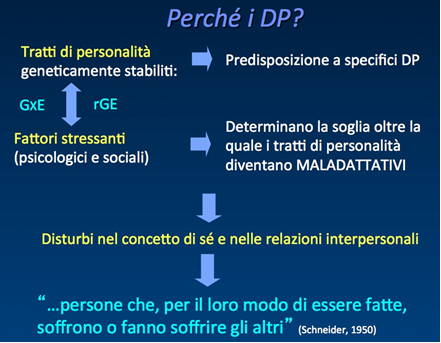
\includegraphics[width=4.26389in,height=2.56250in]{media/image4.png}

Il tutto viene spiegato da due semplici sigle GxE e rGxE.

\textbf{GxE INTERAZIONE GENE-AMBIENTE}

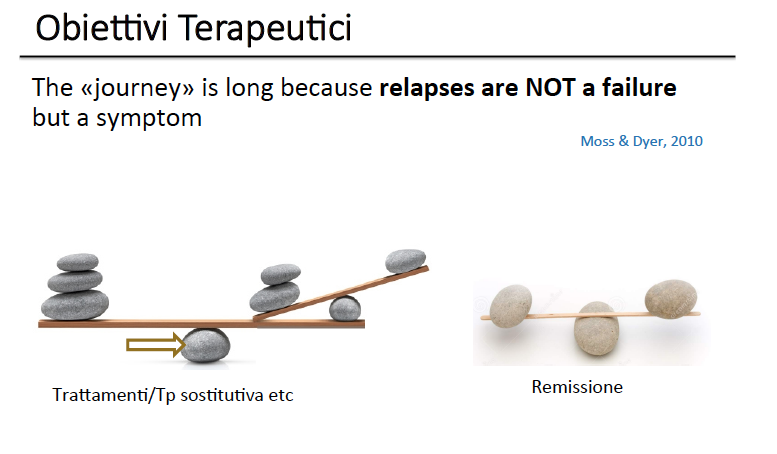
\includegraphics[width=3.68681in,height=2.45833in]{media/image5.png}Non
c'è relazione casuale tra temperamento e ambiente.

Esistono differenze individuali geneticamente modificate nella
sensibilità a specifici eventi ambientali.

Questo spiega bene la questione dell'abuso, del trauma. Per quanto
l'abuso e il trauma siano dei rischi maggiori per qualsiasi disturbo
psichiatrico, non tutte le persone che lo hanno subito sviluppano in età
adulta un disturbo di personalità o psichiatrico di altro tipo.

Questo vuol dire che noi \textbf{reagiamo agli stimoli in modo diverso}.
Tra di noi ci saranno persone più o meno sensibili.

Dunque la variabilità individuale in risposta ad eventi ambientali
dipende da preesistenti differenze individuali nel temperamento.

La ricerca ha dimostrato che gli individui che hanno buone capacità di
autoregolazione, sono quelli più resilienti nei confronti degli eventi
stressanti. Anche se capitano, ho più probabilità di superarli. Tutte le
varianti maladattative delle tre dimensioni conferiscono una maggiore
sensibilità. Importante fu uno studio genetico pubblicato su science che
andò a vedere la relazione tra abuso sessuale infantile e successivo
sviluppo di \textbf{disturbo di personalità antisociale}. E' un disturbo
gravissimo per cui non c'è cura. Queste persone non guariscono e devono
stare in carcere perchè sono delinquenti, serial killer ecc. Nelle serie
americane, quando disegnano il profilo psicologico del serial killer,
mettono sempre che lui, da piccolo, aveva subito abusi, crudeltà; e
questo è vero. Le persone fredde, senza empatia, che godono nel far
soffrire gli altri e non c'è modo di guarirli, hanno avuto una storia di
crudeltà su loro stessi quando erano piccoli.

Rimane il fatto che non tutti quelli che hanno subito degli abusi o
violenze, dopo diventano antisociali. Lo studio infatti ha fatto vedere
che c'è una sorta di verità: C'è correlazione tra abuso e sviluppo di
personalità antisociale solo nei soggetti che hanno bassa attività dell'
enzima MAO A. Questo dunque è un esempio di interazione gene ambiente.

\textbf{rGxE CORRELAZIONE GENE-AMBIENTE}

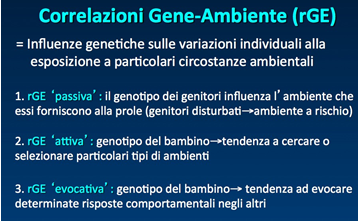
\includegraphics[width=3.72847in,height=2.31250in]{media/image6.png}E'
ben diverso dall'interazione gene ambiente citata prima.

Ci dice che esistono influenze genetiche sulle variazioni individuali
all'esposizione a particolari circostanze ambientali.

Non è semplicemente che io sono diverso da un altro nella mia
sensibilità agli eventi stressanti, ma sono diverso anche per come mi
espongo agli eventi stressanti.

Esistono 3 tipi di correlazione gene-ambiente:

\begin{enumerate}
\def\labelenumi{\arabic{enumi}.}
\item
  \textbf{rGxE ``PASSIVA'':} \emph{Il genotipo dei genitori influenza
  l'ambiente che essi forniscono alla prole.} Pensiamo al 2\^{} caso
  clinico: la madre ha avuto la figlia da giovane. Il padre biologico
  della bambina l'aveva lasciata e da li, la donna ha avuto numerosi
  partner violenti di breve durata e questi abusavano della figlia.
  Quello che noi vediamo è che la ragazza da grande ha un disturbo
  borderline di personalità. Questo è l'effetto del fatto che è
  cresciuta in un ambiente a rischio o è l'effetto del genotipo della
  madre che si è comunque trasmesso a lei? Entrambe le cose. La ragazza
  ha ereditato un genotipo predisponente dalla madre e vivendo in un
  ambiente a rischio ha fatto tracimare le cose. Se ho un genitore
  disturbato è verosimile che io erediti i suoi geni. Però centra anche
  l'ambiente perché i genitori non solo mi hanno passato un genotipo
  predisponente, ma mi hanno tenuta in un ambiente problematico, pieno
  di eventi stressanti. Non è casuale che io abbia una predisposizione
  genetica e mi trovi a vivere in un ambiente già pericoloso per il
  rischio di sviluppare il disturbo di personalità.
\item
  \textbf{rGxE ``ATTIVA'':} \emph{Il modo in cui io sono fatta
  geneticamente, mi predispone a cercare nel mondo e a selezionare
  alcuni tipi di ambiente.} Sempre l'esempio di prima, fa vedere che la
  ragazza già alle medie marina la scuola, viene espulsa e dunque
  abbandona la scuola stessa. In seguito entra in un gruppo di gente che
  si droga ed inizia a prostituirsi per avere eroina. Le relazioni a
  rischio già nell'adolescenza, come avere amici drogati, sono un grosso
  fattore di rischio per i disturbi di personalità, ma anche in questo
  caso il fatto non è casuale. La ragazza era così impulsiva che gli
  stimoli normali, di una classe delle medie, non le bastavano; doveva
  andarne a cercare altri fuori. \emph{La ragazza, a causa del suo
  temperamento, ha attivamente cercato degli ambienti a rischio.}
\item
  \textbf{rGxE ``EVOCATIVA'':} \emph{Il genotipo del bambino causa la
  tendenza di evocare certe risposte comportamentali negli altri.} La
  ragazza quando era a scuola, faceva tanta confusione che è stata
  espulsa. Ha perso un fattore protettivo. Andare a scuola vuol dire che
  si è in grado di seguire le tappe evolutive normali di una persona.
  Lei però evocava negli insegnanti o negli amici ``bravi'' una reazione
  di espulsione. Più avanti evoca la reazione di espulsione nei
  partners: prima li cerca e poi si comporta in modo così caotico che
  tutti la lasciano.
\end{enumerate}

\begin{quote}
Prendiamo come altro esempio il 3\^{} caso clinico: donna con
agorafobia. La donna è nata da genitori già avanti con l'età. Questi
erano iperprotettivi nei confronti della bambina. Non è che non le
volessero bene, ma le dicevano sempre stai attenta, non fare...ecc.
Tendevano a controllarla perché non diventasse troppo autonoma. Anche in
questo esempio possiamo trovare le varie interazioni gene ambiente.

rGxE PASSIVA: siccome i genitori la limitavano molto, si è creato un
ambiente ristretto. La bambina ha avuto paura a cercare cose oltre la
famiglia. Questa cosa non è casuale perché lei ha anche ereditato geni
dai genitori nella tendenza verso la paurosità. Poi i genitori non
l'hanno stimolata a cercare cose nuove, ma anzi le aumentavano la paura.
La ragazza è stata sempre in casa: elementari, medie, superiori. Non ha
mai avuto amici ed i genitori non si sono preoccupati di questo, perché
per loro andava bene così. La ragazza era molto isolata. Loro non hanno
fornito occasioni di novità alla figlia.

rGxE ATTIVA: Il suo genotipo ha fatto si che lei si trovasse il marito
all'interno della cerchia ristretta di famiglia e gli unici amici che
avesse fossero anch'essi in famiglia. Anche il lavoro che faceva era col
marito. La persona ha selezionato nel tempo delle esperienze che
amplificano la sua predisposizione.

Siamo abituati a pensare: l'ambiente ci rende diversi. In realtà, per
come simo fatti, noi plasmiamo l'ambiente a nostra immagine e
somiglianza.

rGxE EVOCATIVO: I ragazzi alle medie la escludevano perché era
perfettina a scuola, però aveva paura degli altri. I bambini l'avevano
emarginata e questo aveva fatto si che venisse meno un fattore
protettivo per lo sviluppo di amicizie sane. Altra cosa importante è che
il marito la lascia perché, pur essendo entrambi andati in pensione, lei
non si sente di andare in vacanza con lui. E' così inibita che non
riesce a fare una cosa che per la maggior parte delle persone è normale.
\end{quote}

\textbf{\emph{TRANSFERT E CONTROTRANSFERT}}:

L'ambiente non è indipendente dalla persona, ma è piuttosto un prodotto
tra interazione di fattori genetici e precedenti eventi ambientali. In
particolare, pazienti con disturbo di personalità, creano l'ambiente a
cui rispondono. Questo paradossalmente mantiene se stessi e l'ambiente
stabili. In tutti i casi che abbiamo visto, i pazienti continuano sempre
a commettere gli stessi errori.

Ciò vuol dire che i fattori di rischio genetici e ambientali non è che
si sommano e basta tra di loro, ma continuano ad essere attivi nella
vita di tutti i giorni. Ci sono alterazioni stabili che continuano ad
alimentare quell'ambiente.

I pazienti con disturbo di personalità non vedono le cose come davvero
stanno. Le loro visioni sono distorte in base al loro mondo interno.
Sembra che i pazienti siano condannati a ripetere i comportamenti del
passato , malgrado la situazione sia nuova, diversa o cambiata. Anche in
un contesto di accudimento (per es il reparto dell'ospedale), la donna
dell'esempio di prima, ripete i comportamenti del passato come se le
stessero facendo del male. Scappa, crea problemi, ci prova con gli
infermieri.

Questa è una cosa che gli psicanalisti chiamavano \textbf{TRANSFERT} (il
mondo interno del paziente induce una distorsione del mondo esterno):
condizione a cui siamo condannati che ci porta a ripetere gli
atteggiamenti del passato. Lo riconosciamo in ogni riposta o
atteggiamento del paziente che differisce dalla risposta ordinaria che
sarebbe attesa in analoghe circostanze da ogni individuo.

Nei disturbi di personalità bisogna chiedersi che cos'è che c'è di
diverso dalla normalità, da quello che ci si aspetterebbe normalmente.
Il transfert si riconosce anche da cose subdole. Lo psichiatra fissa un
appuntamento ed il paziente non ci va. La persona normale se dovesse
avere un contrattempo avvisa. Il paziente con disturbo di personalità
non va agli appuntamenti prefissati e non avvisa. Poi però accade
qualcosa e si presenta in pronto soccorso. Vogliono essere aiutati
subito, fanno confusione, spesso si presentano in condizioni disastrose.
Loro non sono abbandonati, ma si comportano come se lo fossero.

Il fatto di distorcere le relazioni sociali, non lo avvertono come un
problema. Non si rendono conto che quella non è l'usuale norma di
comportamento tra le persone. Per esempio sono persone che, se hanno un
lavoro, ci vanno vestiti in modo inappropriato. Sono quelli che trattano
male i colleghi o i superiori, li accusano di non dare abbastanza
attenzione o ancora quelli che arrivano cronicamente in ritardo.

Quando noi facciamo cose di questo genere, siamo preoccupati di ciò che
causiamo negli altri o a noi stessi, loro no. Quindi lo psichiatra non
può contare sull'alleanza terapeutica con questi pazienti. Dunque se un
paziente con disturbo di personalità inizia a trattarvi nel modo
corretto, come le norme educative tra persone insegnano, vuol dire che
questo è guarito. Come corollario c'è da dire che, siccome questo è il
comportamento di questi pazienti, noi non riusciamo a rimanere
indifferenti. Se uno fa il medico ed una persona continua a non andare
agli appuntamenti, poi si presenta in urgenza andando a dire che non si
fa nulla per lui, lo psichiatra si arrabbia o si sente frustrato; è come
se avesse fallito. Qualsiasi sia il sentimento, prova un sentimento
\emph{indotto} dal comportamento del paziente; non rimane indifferente.

Si deve dunque stare attenti a come reagiamo, cioè al
\textbf{CONTROTRANSFERT}. Questo è il contraltare del transfert del
paziente.

\begin{quote}
\emph{Transfert del paziente}: lui fa sempre le stesse cose malgrado la
situazione non lo richieda più.

\emph{Controtransfert del medico}: il fatto che il paziente faccia una
confusione non giustificata, causa nello psichiatra delle reazioni, che
sia fallimento e frustrazione o rabbia. Il paziente con disturbo di
personalità induce nei medici tipiche reazioni dettate dalla stessa
patologia del paziente. Prima abbiamo visto la stessa cosa e l'abbiamo
chiamata in altro modo: rGxE EVOCATIVA. Per come io sono fatta, evoco
determinate reazioni comportamentali e ambientali negli altri.
\end{quote}

Con il controtransfert corriamo il rischio di reagire in modo tale da
causare una reazione espulsiva e quindi peggiorare la situazione per il
paziente. Si aggiunge un nuovo fattore stressante ed il ciclo si
perpetua. Ci dobbiamo accorgere di essere in preda al controtransfert
(che c'è sempre perché sempre dev'essere presente il transfert,
altrimenti non c'è disturbo di personalità). Tutte le volte che sentiamo
la tentazione di deviare da un trattamento stabilito, da quello che
dovremmo fare in un'analoga situazione, quello è un indice del fatto che
noi stiamo mettendo in atto un azione di controtransfert.

Controtransfert è tutto quello che devia da quello che normalmente
sarebbe atteso da parte del medico. Sentirsi frustrato e impotente o
arrabbiato è un'azione di controtransfert perché in ogni caso non
adempiamo al compito di aiutare il paziente. Nella pratica tutte le
volte che sentiamo un affetto molto intenso nei confronti di questi
pazienti (cioè sempre), anche quando l'affetto sembra particolarmente
buono, come il sentirsi frustrato, in questo caso è meglio stare zitto,
non fare nulla per non mettere in atto la correlazione gene ambiente
evocativa.

Prendiamo l'esempio della ragazza ricoverata che fa amicizia con tutti e
ci prova con l'infermiere. Questo è un transfert, non è una cosa
normale, perché devia da quello che ci si aspetterebbe in analoghe
circostanze. L'infermiere come si è sentito? Sicuramente imbarazzato, ma
anche lusingato. Quando mettiamo questi pazienti in un reparto con tanti
operatori, succede che alcuni dicono che la odiano, non gli piace, è la
solita psicopatica; altri dicono che è intelligente, che ha avuto tante
sfortune nella vita, ha lavorato tanto.

Il transfert di questa persona nei diversi operatori è mutevole, perché
mutevole è il mondo interno della paziente. Anche il controtransfert
dunque sarà diverso a seconda dell'operatore. Ci sarà chi avrà una
reazione espulsiva e chi ha reazioni del tipo `` io ti salverò''.
L'infermiere si è comportato nel modo giusto, ma poteva anche mettersi a
parlare con questa paziente più che con altri. Questo non è un problema
riguardo il fatto che la scelta sia giusta o sbagliata, ma ci dice
qualcosa di importante del paziente. Dedico più tempo a lei perchè mi
sento lusingato e questo è già un' espressione di controtransfert.

Al di la del transfert che fa il paziente con disturbo di personalità,
il controtransfert come definizione generale dipende da tante cose. Per
esempio, dipende da come ci si alza al mattino, dai problemi che si
hanno a casa o in famiglia, da come si è fatti caratterialmente (ci sono
persone che vedono tutto positivo, altre tutto negativo).

Quindi il controtransfert è dettato molto anche dalle caratteristiche
del terapeuta. A ciò si aggiunge il transfert del paziente. In generale
però le caratteristiche proprie della personalità del terapeuta vengono
in secondo piano perché è cosi potente il transfert del paziente che
tutto il resto è secondario. Quindi è importante capire le nostre
reazioni affettive perché sono diagnostiche. Ogni volta che ci troviamo
a parlare con un collega di un paziente ed abbiamo opinioni totalmente
discordanti, allora quello è controtransfert e quello è un disturbo di
personalità.

\emph{Analizziamo nel dettaglio i diversi tipi di disturbo della
personalità:}

\textbf{\emph{CLUSTER A:}}

\begin{itemize}
\item
  \textbf{\emph{DP SCHIZOTIPICO:}}
\end{itemize}

Non si hanno deliri o allucinazioni, altrimenti parleremmo di veri e
propri disturbi psicotici. Gli schizotipici però hanno dei sintomi
simil-psicotici, come:

\emph{pensiero magico,}

\emph{dee di riferimento} (sensazione che le cose intorno hanno a che
vedere con me),

\emph{illusioni ricorrenti,}

\emph{linguaggio strano o metaforico o addirittura allusivo}.

L'affettività è inappropriata o coartata (non c'è tutta la varietà delle
risposte emotive che normalmente dovrebbero esserci; spesso cambiamo
emozione in base a ciò che capita, in questo disturbo no). Inappropriata
è qualcosa di più: ho un'emozione di un tipo in una circostanza che ne
richiederebbe tutt'altra, tipo ridere ad un funerale. Questi pazienti
provano DISAGIO ACUTO quando stanno con gli altri. Il paziente di questo
tipo non è violento, ma se pressato dagli altri sta malissimo e può
diventare irritabile. Questo disagio non diminuisce con la familiarità.
Non sto male in mezzo a persone che non conosco e quando ci divento
amico il disagio passa. A questi pazienti il disagio non passa.

\emph{\emph{L'anamnesi personale è ricca di deficit sociali ed
interpersonali. }}

C'è una mancata richiesta di trattamento perché non c'è consapevolezza
di malattia. In generale nei disturbi di personalità non c'è mai
consapevolezza di averla perché ``io sono fatto così''si parla di
egosintonia. Non è che va male come sono fatto, se mai sono gli altri
che non mi capiscono. Spesso sono obbligati a chiedere aiuto dai
familiari, per la loro stranezza. Il DP schizotipico è un po' strano
rispetto agli altri, tanto che la classificazione attuale li colloca sia
tra i DP, sia nei disturbi psicotici. Questo infatti può costituire il
prodromo della schizofrenia.

\emph{Studio}:Si è fatto uno studio molto rilevante a riguardo. È
incominciato tra gli anni `50/'60 in Danimarca (studio danese sugli
adottivi). L'obiettivo era vedere qual' era la prevalenza di
schizofrenia o disturbi affini nei familiari di 1\^{} grado (padre e
madre) biologici ed adottivi di bambini adottati nelle prime settimane
di vita, che da adulti avessero sviluppato schizofrenia. Cos'è che
predispone alla schizofrenia: la genetica o l'ambiente? Sono partiti
negli anni `60 e sono andati a vedere il registro delle adozioni intorno
agli anni `40. Hanno cercato tutte le persone che, adottate tra 1924 e
1947, da grandi, cioè nel 1960, avessero la schizofrenia. A partire da
14427 adottati, hanno identificato 42 pazienti schizofrenici e poi hanno
valutato i controlli, cioè 42 persone che non avevano sviluppato la
malattia. Il passaggio successivo è stato riprendere il registro delle
adozioni e vedere chi erano i familiari biologici e chi i familiari
adottivi. Hanno poi riguardato il registro psichiatrico per vedere qual'
era la prevalenza di schizofrenia in entrambe le categorie. Alla fine
per essere sicuri, hanno preso le interviste fatte a ciascuno, e le
hanno mandate in America, dove la società degli psichiatri americani
stava mettendo a punto una delle prime edizioni del manuale diagnostico
e statistico dei disturbi mentali (DSM III). Hanno fatto fare loro una
valutazione indipendente. Lo studio ha dato come risultato che la
prevalenza di schizofrenia era a livello dei familiari biologici di
bambini adottivi che da grandi avevano sviluppato la schizofrenia. La
prevalenza in questo caso era del 5\% a fronte di uno 0,4\% di
prevalenza nei genitori adottivi. Si è visto poi che c'è anche una
maggior prevalenza di schizofrenia latente o disturbo schizotipico di
personalità nei familiari biologici rispetto ai familiari adottivi (11\%
CONTRO 2\% DEI FAMILIARI ADOTTIVI). Questo vuol dire che \emph{quello
che si eredita è proprio il disturbo schizotipico di personalità. Poi
uno se lo può tenere così tutta la vita o può sviluppare schizofrenia.}

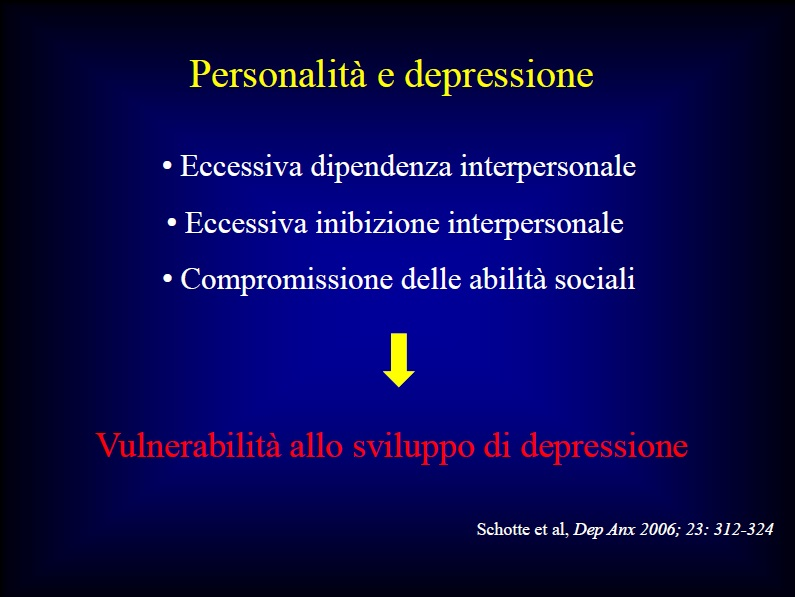
\includegraphics[width=3.81250in,height=1.56250in]{media/image7.jpeg}Questo
invece è un articolo che suddividere le personalità borderline con la
schizofrenia borderline. Da una parte c'è il disturbo di p.
schizotipico, dall'altra ci sono tutti gli altri disturbi di personalità
in cui vanno a ricadere tutte le forme di schizofrenia pseudonevrotica o
borderline. Quindi il disturbo schizotipico è molto diverso dagli altri
disturbi.

\begin{itemize}
\item
  \textbf{\emph{DP PARANOIDE:}}
\end{itemize}

E' un disturbo PERICOLOSO che non conduce allo stesso distacco sociale
dello schizotipico (che sta male nelle situazioni sociali), ma ad un
distacco sociale dettato dal fatto che è dovuto alla convinzione
pervasiva di essere sfruttati, ingannati o danneggiati.

Si caratterizza infatti per pervasive sfiducia e sospettosità verso gli
altri. Sono persone che dubitano o pensano in maniera ricorrente che gli
altri vogliano ingannarli, fargli del male, tradirli. Questo è il loro
modo di rapportarsi con gli altri. Questo può essere definito mondo
esterno. Anche in questo caso quello che vedremo è un apparente distacco
sociale, ma a differenza dello schizotipico che, se messo in mezzo agli
altri, sta male perché ha un disagio acuto, il paranoide è
apparentemente distaccato perché ha una riluttanza a confidarsi.

Non è un delirio o allucinazione. Non hanno neanche un vero delirio di
persecuzione. L'ambiente è percepito in modo preciso, ma nella vita
quotidiana attribuiscono un significato distorto a quello che pur
correttamente vedono nell'ambiente. Il significato distorto è sempre nel
senso: ``ce l'hanno con me''. In qualsiasi relazione o contesto in cui
si trovano, vanno alla costante ricerca di significati oscuri. C'è
infatti iperattivazione dell'attenzione e sono molto tesi. Sono persone
che vanno in giro molto attente per captare tutti i significati nascosti
nelle parole o nei comportamenti della gente. Quello che capita nel
mondo interno di questi pazienti è qualcosa che si chiama proiezione. È
un meccanismo di difesa per cui ``io non sono cattivo, non sono
arrabbiato con nessuno'', ma lo faccio perché proietto tutto quello che
ho di negativo dentro di me sugli altri, che diventano cattivi e
persecutori. Non sono consapevole di questa cosa.

Quello che capita ai pazienti con questo disturbo è che rispondono con
rabbia a qualsiasi cosa gli si dica. Percepiscono come attacchi
qualsiasi osservazione, anche se neutra.

Hanno molto bisogno di controllare gli altri e non sopportano il
controllo altrui. Qui il transfert sarà il sospettare degli altri anche
se loro fanno il loro lavoro. Nessuno è esente da questa situazione. I
pazienti con DP paranoide sono tra i pazienti più pericolosi perché se
la prendono con tutti, nessuno è esente.

Sono pazienti che intentano cause contro medici, direzione sanitaria;
sono quelli che scrivono perché si sentono curati ingiustamente, vi
portano in tribunale ecc. Di solito un paziente di questo tipo va dallo
psichiatra perché obbligato. In genere perché gli sono successe diverse
cose. Ad esempio il paziente si sposa, ma la moglie lo lascia perché è
un geloso patologico, le controlla tutto. Se lei cerca di allontanarsi,
lui diventa stalker. Ci sono frequenti liti che lui non vede come frutto
di un suo disturbo, ma dovute al fatto che lei non gli voglia abbastanza
bene.

Altro motivo per cui un paziente così va dallo psichiatra è perché ha
già fatto 8 cause di mobbing nei confronti dei datori di lavoro, o è
stato più volte licenziato, o si è auto licenziato perché si è sentito
trattato ingiustamente dal punto di vista della collocazione lavorativa.
Tutto questo non perché lui ha fatto qualcosa che non va, ma perché gli
altri non hanno capito il buono che c'è in lui. Dunque se va dallo
psichiatra, al massimo è per depressione. La diagnosi di DP paranoide
però viene messa dopo 6 mesi, non perché non si capisca il tipo di
paziente, ma perché fargli accettare questa patologia è difficilissimo.
Quando arriva dallo psichiatra in genere porta dei plichi pieni di
cartelle che contengono in modo dettagliato tutta la storia delle sue
sfortune, spesso sanitarie. Comincerà a parlare male di tutti i medici
che in passato l'hanno visitato e mostrerà referti, spesso messi in
ordine alfabetico e numerati, per convincervi di quanto gli altri lo
abbiano trattato o curato male. Dunque sono pazienti che ricercano
puntigliosamente chi e dove possa avere sbagliato in qualcosa e nel caso
della sanità spesso iniziano a denunciare una serie di volte i possibili
colpevoli, poi si rivolgono al tribunale del malato e se anche questo
non dovesse bastare agiscono direttamente usando violenza fisica o
verbale su chi di dovere.

\emph{Caso Clinico}: \emph{Un esempio eclatante è quello di una donna
che, dopo che è stato scoperto al marito un tumore al polmone, è andata
a cercare ogni particolare nelle visite precedenti per capire se
qualcuno non avesse potuto scoprire prima la neoplasia del coniuge. Alla
fine ha mandato delle lettere ai medici minacciandoli che se il marito
fosse morto loro stessi avrebbero fatto un suicidio a due. Era decisa
inoltre a mandare una lettera al tribunale per far cadere la colpa sui
medici. Quindi li ha ricattati.}

Queste persone sono molto pericolose anche sul lato personale,
sentimentale. All'inizio fanno sentire il compagno o la compagna molto
bene, piena di attenzioni, al prezzo che però lui/lei facciano
esattamente ciò che gli si dice. E questo per loro non sarà mai
abbastanza. Anche andare a bere il caffè con un amico, può essere segno
di qualcosa che non va, di un tradimento.

Il controtransfert è all'inizio impazienza, poi reazioni difensive man
mano che riconosciamo il tipo di problema.

\emph{\emph{L'anamnesi personale è instabilità lavorativa, rotture
relazionali, vicende giudiziarie, lite con i sanitari di riferimento. }}

Dove sono i criteri generali di disturbo di personalità? Queste persone
funzionano molto male in ogni settore. Non sanno accordare i loro
comportamenti in base ai loro obiettivi, che è qualcosa che riguarda il
sè, perché non riescono a tenere un lavoro ad esempio, in quanto si
sentono perseguitati. Poi c'è instabilità interpersonale sempre per la
stessa causa. Dunque è presente il criterio cardine per i DP. C'è una
disfunzione nell'area del sè e nelle relazioni interpersonali.

La psichiatria classica dice che il DP paranoide può predisporre a
paranoia, ma dati certi non ce ne sono.

\begin{quote}
Il confine con la paranoia, che possono avere anche soggetti sani, è che
in questa non c'è un franco delirio di persecuzione. Si è visto inoltre
che se un individuo con disturbo paranoide ha un altro disturbo di asse
1 (disturbo dell'umore, depressione maggiore ricorrente), il DP
preesistente è \textbf{patoplastico} nei confronti del secondo disturbo
(episodio depressivo) e come conseguenza, durante l'episodio depressivo
maggiore è più probabile che il paziente abbia episodi paranoici più
gravi dei soliti.
\end{quote}

\begin{itemize}
\item
  \textbf{\emph{DP SCHIZOIDE:}}
\end{itemize}

Si caratterizza per un \textbf{marcato distacco nelle relazioni sociali
per indifferenza alle stesse}, e di pazienti sperimentano in genere una
\emph{gamma ristretta di emozioni nei contesti interpersonali},
rispondendo con \emph{indifferenza quasi assoluta alle lodi o alle
critiche degli altri}. In poche parole, il paziente si presenta come un
soggetto solitario, che vive la sua vita distanziando gli altri. Ha un
distacco nelle relazioni sociali per indifferenza alle stesse.

Di questi disturbi se ne vedono pochissimi, perché non vanno dallo
psichiatra e se ci vanno sono ben riconoscibili: sudatissimi, mutacici,
incapaci di stare fermi e incapaci a rispondere altro che si o no.

Esperiscono una ristretta gamma di emozioni nei contesti interpersonali.
Rispondono con indifferenza alle critiche o alle lodi altrui.

Nella vita il paziente va avanti distanziando gli altri (correlazione
gene ambiente evocativa). \emph{\emph{L'anamnesi personale è isolamento
sociale e mancata richiesta di trattamento, perché un paziente di questo
tipo non ha i sintomi bizzarri dello schizotipico che prima o poi lo
portano all'attenzione clinica. }}

\begin{quote}
Quindi è rarissimo nella pratica clinica. Anche qui rimane la possibile
relazione con la schizofrenia. Mentre la schizoidia è generalmente più
vicino alla schizofrenia, il DP schizoide non si sa bene in che
relazione sia con la schizofrenia. A volte la fase residuale della
schizofrenia (senza allucinazioni o deliri) assomiglia alla Schizoidia.
\end{quote}

\textbf{\emph{TERAPIA NEI DP DI CLUSTER A}}

Per quanto riguarda la \textbf{\emph{terapia}} dei clusters di tipo A,
essendo questi quelli maggiormente correlati coi sintomi schizofrenici,
sono anche i DP che \emph{rispondono meglio alla terapia farmacologica},
che si avvale essenzialmente di \textbf{antipsicotici di seconda
generazione} (clozapina, olanzapina, quetiapina) \emph{a basse dosi}.

Il principali problema, tuttavia, risiedono nel:

\begin{itemize}
\item
  \emph{convincerli ad assumere i farmaci}, perché i pazienti
  (soprattutto i paranoici) non ritengono di essere malati,
\item
  inoltre il medico deve sempre \emph{evitare di cedere ad un meccanismo
  di controtransfert}. Cerchiamo di stare il più possibile tranquilli.
  Bisogna capire cosa si sta sentendo, quale sia la relazione normale
  medico-paziente. Perché si potrebbe avere la tentazione di dire che
  quelli prima di noi non hanno capito nulla ed ora noi riusciremo a
  risolvere i problemi. Più attenzioni gli diamo, più questo tipo di
  paziente si accanirà contro di noi dopo (quello che da medici potremmo
  essere tentati di fare è il Controtransfert complementare). Evitare
  atteggiamenti amichevoli che nei confronti di un DP paraoide potrebbe
  essere è il modo migliore per farsi ammazzare dal paziente, che spesso
  si convince che il medico è gentile con lui perché vuole ingannarlo,
  per cui spesso arriva a colpirlo alle spalle.
\item
  Il disturbo schizoide è molto difficile da trattare perché significa
  essere di fronte ad assenza di relazione medico paziente
\end{itemize}

Quindi bisogna non subito aggedire il paziente con diagnosi e terapie
(il problema è convincerli a prendere i farmaci) e non discutere le
verità del paziente all'inizio..

\textbf{\emph{CLUSTER B:}}

\begin{itemize}
\item
  \textbf{\emph{DP ANTISOCIALE:}}
\end{itemize}

Questo disturbo è facilmente riscontrabile in carcere e molti di quelli
che si vedono ricoverati in psichiatria non dovrebbero starci.

Nela storia di questi pazienti ci deve essere obbligatoriamente un
disturbo della condotta in adolescenza. Per disturbo di condotta si
intende che prima dei 18 anni di età si abbiano comportamenti teppisti.
Sono comportamenti crudeli verso cose, animali o persone.

Si parla di devianza dalle regole, abuso di sostanze fin dalla tenera
età, marinare la scuola, atti di crudeltà gratuita.

Non tutti i disturbi di condotta diventano DP antisociale, ma tutti i
pazienti con DP antisociale lo hanno avuto prima dei 18 anni (prima di
questa età non si può fare diagnosi).

Si caratterizzano per \textbf{pervasiva inosservanza e violazione dei
diritti altrui} (alla libertà, alla vita ecc); fanno questo senza dare
importanza ai loro atteggiamenti.

Presentano una totale \textbf{assenza di empatia}, non si pentono o
vergognano e non hanno rimorsi. Questo loro non lo impareranno mai. Loro
capiscono molto bene di aver fatto dei danni ad una persona, ma non gli
importa nulla, o addirittura ne sono gratificati.

Non ci sono terapie per insegnare ad entrare in empatia. Anzi più fanno
terapia, più peggiorano\emph{. \emph{L'anamnesi è di carcerazioni e di
comportamenti illeciti e violenti, spesso associati ad abuso di
sostanze.}}

I disturbi di personalità non sono come la schizofrenia. Non è che
questi pazienti non sono responsabili di quello che fanno. Hanno dei
disturbi seri, però non compromettono mai totalmente la capacità di
cambiare il loro comportamento, se aiutati a farlo. Da ciò ne consegue
che questi disturbi, così come li descriviamo, non compromettono la
capacità di intendere e volere. L'antisociale \textbf{sa perfettamente
che sta commettendo un reato}. Non è come uno schizofrenico che in preda
ad un'allucinazione uccide la madre e in quel momento non era capace di
intendere e volere.

Se uno ha disturbo di personalità antisociale o paranoide dovrebbe
andare in galera, se colpevole. Ultimamente però ci sono state due o tre
sentenze in cui un perito ha dichiarato non imputabile un paziente con
DP. Se passa questa linea è un problema perché oltre a ``giustificarli''
non si prova neanche a curarli.

\begin{itemize}
\item
  \textbf{\emph{DP NARCISISTICO:}}
\end{itemize}

Si caratterizza per \textbf{pervasive grandiosità nella fantasia o nel
comportamento} (non stiamo parlando del narcisismo sano).

Nella fantasia vuol dire che il paziente fuori è timido e magari fa
complimenti agli altri, ma dentro di se si sente il \textbf{migliore in
ogni cosa}, anche nella sfortuna.

Si riscontrano \textbf{necessità di ammirazione} e \textbf{mancanza di
empatia}. E' un po' simile all'antisociale con cui a volte ci sono dei
tratti almeno in comorbidità, mancanza di empatia ( la preoccupazione
per gli stati d'animo altrui ).

Nel mondo interno del paziente conta una sola cosa: come faccio ad avere
sempre una stima di me altissima.

Questi pazienti sono estremamente \textbf{sensibili alle critiche}
altrui perché interpretano qualsiasi cosa come una minaccia alla loro
autostima. In inglese questo viene definito \textbf{``entitlement}'':
ogni cosa è dovuta, diritto. E' come se il feedback positivo degli altri
non fosse mai abbastanza.

In questo senso è come se gli altri non avessero bisogni propri. Gli
altri esistono, ma non in quanto persone separate da me, con loro
bisogni e aspettative, ma \textbf{gli altri} esistono ed io li tratto
bene solo se \textbf{servono a sostenere la mia autostima}.

Gli uomini con DP narcisistico vorranno donne belle, che pendono dai
loro occhi e loro serviranno solo finchè assolvono alla loro funzione.
Se non assolvono più, non c'è modo di farli tornare ad amare quella
persona. Infatti i soggetti con questo disturbo hanno incapacità di
amare, di avere relazioni reciproche e mutualmente appaganti.

C'è solo un \textbf{``do ut des'':} se faccio qualcosa per te, lo faccio
solo perché tu mi dai qualcos'altro. Non lo faccio per gratuità, perché
ti voglio bene.

La letteratura psicodinamica identifica due tipi di DP narcisistico:

\begin{quote}
1.grandioso e arroganteOVERT;

2.ipervigile ed ansioso che dentro di sé ha malattie di grandezzaCOVERT.
\end{quote}

In realtà oggi si dice che queste caratteristiche coesistano nello
stesso paziente, che non siano divise.

\emph{\emph{Nell' anamnesi di questi pazienti ci sono difficoltà
relazionali e coniugali e nella media età-adulta, disturbi depressivi a
volte molto seri. }}

Spesso ci sono casi di suicidi in persone di 40/50 anni che non hanno
mai avuto niente. Questa potrebbe essere la storia tipica di un DP
narcisistico. Sono persone che pensano di avere tutte le capacità del
mondo, aspettano che succeda qualcosa, pensano di avere tutto il tempo
che vogliono. Credono di potersi permettere di non fare le cose che
fanno gli altri, come stare su un banco, studiare o lavorare.
Tipicamente appaiono molto affascinanti. Hanno una serie di relazioni
nelle quali all'inizio c'è grande coinvolgimento, perché sostengono
molto l'altro partner. Devono farlo stare molto bene perché questo fa
stare bene loro, poi lo buttano via quando questo finisce e tutto
ricomincia da capo. Si trovano a 42/43 anni di fronte alla realtà: tutti
hanno un lavoro avviato, fanno le loro cose, hanno figli, una relazione.
Questo per loro è il momento più duro, dove c'è rischio di grave
depressione e possibilità di suicidio. È molto difficile curarli in
questo momento.

Il disturbo narcisistico di personalità si può presentare in modi
differenti ed è talmente complesso che alle volte può essere difficile
diagnosticarlo.

Discutiamo alcuni casi clinici:

\begin{enumerate}
\def\labelenumi{\arabic{enumi}.}
\item
  \emph{Mister A è un uomo di 42 anni che si presenta ad uno
  psicoterapeuta privato ed il motivo per cui lo fa sono dei problemi
  con la moglie. L'uomo è un imprenditore di successo, molto
  competitivo. Descrive di essere molto socievole e stare con gli altri.
  Quando è in mezzo alle persone riferisce di aver bisogno di essere al
  centro dell'attenzione. Gli piacciono molto le sfide al lavoro dove
  crede di avere possibilità maggiori degli altri nel vincerle. Va in
  trattamento perché si sta chiedendo se finire o meno il suo
  matrimonio. Egli dice di aver perso l'interesse sessuale nei confronti
  della moglie. Durante tutto il matrimonio ha mantenuto una serie di
  amanti e poi le ha sostituite con altre dopo poco che le frequentava.
  Se gli si chiede come mai ha avuto questo comportamento, lui risponde
  che questi non sono problemi legati al suo matrimonio, ma sono
  situazioni proprie, personali.} Questo, anche se difficile da
  identificare, è un DP narcisistico.
\end{enumerate}

\begin{quote}
Se osserviamo meglio vediamo che i problemi sono:

\textbf{mondo interno}Il paziente si sente superiore a tutti gli altri
nel lavoro;

\textbf{mondo esterno} il paziente sta bene con gli altri, ma solo nella
misura in cui l'altro serva per esaltare ulteriormente la sua persona.

Sul lavoro questa persona funziona, anche se abbiamo detto che con
questo disturbo si dovrebbe avere un disfunzionamento in tutte le aree.
Il motivo per cui l'area lavoro apparentemente funziona, è che i
rapporti con i colleghi ed il lavoro stesso sono improntati sul
mantenere al centro dell'attenzione il paziente stesso. Questo è un
esempio di DP ad alto funzionamento. Tutto ruota intorno a lui, gli
altri non hanno bisogni propri ma servono solo per mantenere la propria
autostima.
\end{quote}

\begin{enumerate}
\def\labelenumi{\arabic{enumi}.}
\item
  \emph{Mister B è un uomo single di 32 anni. Ha una storia di abuso di
  alcool e cocaina ed è disoccupato. Si è presentato in ps lamentando
  dolore dopo una procedura dentale e richiede oppiacei. Lui cerca di
  ingraziarsi il medico di guardia che però, prima di dare il farmaco
  vuole sentire il parere del dentista. A quel punto il paziente ha
  iniziato a minacciare e insultare il dottore, il quale contatta la
  ragazza del paziente. Lei riferisce che di recente ha lasciato mister
  B perché lui stava approfittando di lei economicamente, si stava
  facendo mantenere. L'uomo era stato licenziato un anno prima da un
  lavoro molto ben retribuito, ma da allora non ha trovato nessun lavoro
  che potesse fargli mantenere aspettative alte sul suo conto. Ha
  rifiutato lavori non considerandoli alla sua altezza.}
\end{enumerate}

\begin{quote}
Dove si trovano in questo caso i criteri generali di DP e le
caratteristiche di DP narcisistico?

\textbf{Mondo interno} incapacità a perseguire i propri obiettivi. Io
dovrei lavorare, ma pur di adattarmi alle richieste reali, vado avanti
facendomi mantenere.

\textbf{Mondo esterno} rimane con la fidanzata perché lo finanzia e
serve a mantenere il suo status.

Nella sua anamnesi c'è anche abuso di cocaina e di alcool. Se il
soggetto abusa di sostanze stimolanti, vuol dire che ricerca
gratificazione. La dimensione di temperamento che si associa, se
estrema, a questi stimoli è ``la ricerca di stimoli forti''. L'uomo è
una persona intollerante alla frustrazione.
\end{quote}

\begin{enumerate}
\def\labelenumi{\arabic{enumi}.}
\item
  \emph{Mister C è un ragazzo single di 29 anni. Ha una storia di
  diabete insulinodipendente. Si presenta in ambulatorio psichiatrico
  per fobia sociale e distimia, disturbo dell'umore in senso depressivo
  non così grave da essere catalogato come depressione maggiore. }
\end{enumerate}

\begin{quote}
\emph{Lui ha tenuto una serie di lavori di basso livello che non hanno
mai funzionato. Attualmente lavora part time in un' agenzia per
inserimento dati. }

\emph{Quando si descrive dice che il suo umore è cronicamente miserevole
e facilmente va in crisi. Non trae piacere da nulla e quotidianamente si
chiede se questa vita vale la pena di essere vissuta. Quando si sente
giù di morale, dimentica di somministrarsi insulina e per questo viene
ricoverato spesso per scompensi glicemici. Costantemente si paragona
agli altri. E' invidioso e pieno di risentimento. Si sente come
deficitario e sempre in difetto rispetto agli altri. Ha risentimento
perché gli altri non capiscono quello che lui può offrire. Ha fantasie
ricorrenti sul suo datore di lavoro che potrebbe andare a fare una
conferenza stampa e dire a tutti quale talento abbia mister C; altre
volte ha la fantasia di umiliarlo con dimostrazione delle sue capacità
superiori.}

Qui dov'è il DP narcisistico?

\textbf{Mondo interno}sembra soffrire di più rispetto agli altri del suo
stato interiore. Si sente cronicamente inadeguato e privo di capacità.

\textbf{Mondo esterno} lavori mai andati a buon fine, difficoltà a
relazionarsi con gli altri per fobia sociale.
\end{quote}

\begin{enumerate}
\def\labelenumi{\arabic{enumi}.}
\item
  \emph{Miss D 44 anni, single. Si lamenta di avere depressione
  resistente. Ha invalidità psichiatrica per questo motivo. E' stata
  trattata con tutti i farmaci disponibili incluso l'elettroshock. Parla
  dei medici precedenti in modo svalutante. Sembra quasi gratificata nel
  raccontare che tutti abbiano fallito con lei. }
\end{enumerate}

\begin{quote}
La sua terapeuta di gruppo fa diagnosi di DP narcisistico basandosi sul
gap tra l'immagine che lei ha su se stessa come autrice di libri
estremamente dotata, che ancora non è stata riconosciuta ma la realtà è
che lei non ha scritto nulla. Ci sono anche caratteristiche antisociali
perché mente cronicamente a tutti fregandosene. Ha una storia di
prostituzione quando aveva 20 anni e ha fatto imbrogli per ottenere
disabilità piuttosto che lavorare. Non c'è nessun segno di depressione
endogena. Quando la terapeuta le consiglia di trovare un lavoro, la
signora D afferma che si sarebbe uccisa lei stessa o avrebbe ucciso il
terapeuta se questa cosa avesse interferito con la possibilità di
ottenere l'invalidità. Quando c'è una depressione che non riesce ad
essere curata in nessun modo, bisogna sempre pensare alla presenza
sottostante di un disturbo di personalità.
\end{quote}

\begin{itemize}
\item
  \textbf{\emph{DP ISTRIONICO:\emph{: DP}}}
\end{itemize}

Pattern pervasivo con emotività eccessiva e ricerca di attenzione. I
pazienti esprimono in modo drammatico e con enfasi le proprie emozioni
(si ride o si piange a dismisura).

Hanno un'\emph{Emotività molto intensa}, ma l'espressione delle emozioni
è mutevole e superficiale (cambiano in maniera repentina il tono
dell'umore); facile suggestionabilità (le emozioni si trasmettono al pz:
se una persona piange, anche il pz piange).

Interazione con gli altri: \emph{comportamento seduttivo o provocatorio}
(disturbo istrionico più frequente nelle donne che negli uomini).
Considerano le relazioni più intime di quanto non siano. Superficialità
delle emozioni e mancanza di empatia.

\emph{Esibizionismo non fine a se stesso}, sono proprio avidi delle
attenzioni altrui. Quando non hanno le attenzioni dalle persone che
considerano intime diventano intolleranti alle frustrazioni e
percepiscono facilmente l'abbandono.

\emph{Elevata comorbidità con disturbi somatoformi} (ipocondria,
conversione o isteria, somatizzazione). Sintomi somatici che, però, non
sono in parte o del tutto spiegati da cause medico-organiche.

\emph{Sono egosintonici} quindi è importante osservare il paziente e non
solo ascolatare ciò che dice.

\textbf{\emph{ISTERIA:}}

Disturbo in auge nel 1900, oggi è detto ``disturbo da conversione''. Era
tipica delle giovani donne di buona famiglia che Freud considerava
sessualmente inibite. L'ansia che, secondo Freud, giaceva nell`inconscio
di queste pazienti (dovuta al non poter esprimere l'impulso sessuale)
causava angoscia e senso di colpa. Quando un conflitto diventa più forte
bisogna difendersi ancora di più e allora la semplice rimozione potrebbe
non bastare in quanto l`ansia non è controllata. Intervengono a questo
punto altri meccanismi di difesa e nell'isteria abbiamo dunque la
conversione dell'ansia in sintomi somatici. Le isteriche ai tempi di
Freud avevano delle crisi tonico cloniche in cui mimavano l'atto
sessuale (arco di Charcot). Nonostante tipicamente la conversione
somatica sia a carico del sistema nervoso con pseudo crisi epilettiche
(EEG non alterato, non c'è incontinenza sfinterica, non c'è morsus) vi
sono anche altre manifestazioni: cecità isterica, bolo isterico,
paralisi isterica, mancanza di sensibilità che tipicamente non segue la
distribuzione nervosa (anestesia a guanto o a calza, se coinvolge mano o
gamba).

I disturbi istrionici sono difficili da curare e da diagnosticare:
infatti la diagnosi è di esclusione con EEG in corso di crisi. In genere
si parla di facilità d'organo: se l'ansia deve manifestarsi in qualche
modo sceglierà sempre l'organo in parte compromesso. Non esistono linee
guida da applicare motivo per cui spesso non si sa cosa fare.

\begin{itemize}
\item
  \textbf{\emph{DP BORDERLINE:}}
\end{itemize}

Principe dei disturbi di personalità. Disturbo più studiato per quanto
concerne il trattamento sia farmacologico che, soprattutto,
psicoterapeutico (evidence based).

\emph{INSTABILITA' nelle relazioni interpersonali, nell'immagine di sé,
nell'umore e nell'impulsività.}

\begin{enumerate}
\def\labelenumi{\arabic{enumi})}
\item
  \textbf{Ipersensibilità interpersonale} (es: \emph{questi soggetti,
  qualsiasi cosa si dica in un dato momento, possono percepirla dapprima
  come la cosa più bella ed in un secondo momento come la peggiore}).
  Molto sensibili a tutti gli stimoli interpersonali, anche se
  interpretati in maniera distorta.
\end{enumerate}

\begin{enumerate}
\def\labelenumi{\alph{enumi})}
\item
  Relazioni interpersonali instabili e intense, caratterizzate
  \emph{dall'alternanza tra gli estremi di iperidealizzazione e
  svalutazione} (percezione degli altri o come idealizzati o come invece
  cattivi, malevoli\emph{) e tra ipercoinvolgimento e distacco.}
\end{enumerate}

\begin{itemize}
\item
  \emph{\emph{Scissione intrapsichica}} -- distorsione della realtà. Il
  soggetto controlla l'angoscia dividendo il mondo in due: tutto ciò che
  c `è di buono e tutto ciò che c'è di cattivo. Le persone senza
  disturbo di personalità danno un'immagine di sé e degli altri
  ``complessa'' o meglio ancora integrata, cioè realistica, con
  caratteristiche positive e negative di se stessi e degli altri. I
  pazienti borderline non sanno mettere insieme questi aspetti nella
  stessa persona e nello stesso momento. L'immagine di sé che hanno è: o
  ``io bravissimo'', perché c `è qualcuno di perfetto che mi vuole bene,
  o ``io rifiutato'', perché c `è qualcuno che mi vuole far del male.
  Questi due aspetti di sé non entrano mai in contatto non vedono la
  totalità delle cose, ma solo gli estremi esasperati. Spesso non hanno
  neanche la consapevolezza di aver detto in due momenti cose differenti
  (appunto scissione).
\end{itemize}

\begin{enumerate}
\def\labelenumi{\alph{enumi})}
\item
  Costante preoccupazione e conseguenti sforzi disperati per evitare un
  reale o immaginario abbandono:
\end{enumerate}

\begin{itemize}
\item
  \emph{\emph{Intolleranza alla solitudine o ipersensibilità al
  rifiuto}} comportamenti ``acting out'', cioè sforzi disperati per
  evitare l'abbandono (es: \emph{chiamano la polizia, si tagliano, vanno
  in overdose}). Noi tutti, come esseri umani, abbiamo un sistema
  tramite cui avvertiamo la minaccia di un'esclusione, sistema di
  allarme che ci fa sentire male, il cosiddetto ``dolore sociale''. Il
  dolore allerta le varie aree per dar inizio a meccanismi di
  accettazione in quanto il compito evolutivo dell'uomo è quello di
  stare in gruppo. Questo sistema si può manipolare con diversi
  esperimenti in cui viene riprodotto il contesto di esclusione sociale.
  E' stato visto che i pazienti borderline non stanno male soltanto
  quando sono esclusi, ma anche quando c'è una normale situazione di
  inclusione: percepiscono l'abbandono ovunque \emph{ipersensibili all'
  abbandono}.
\end{itemize}

\begin{enumerate}
\def\labelenumi{\alph{enumi})}
\item
  Sentimenti cronici di vuoto; alterazione dell'identità; senso di
  percezione di sé marcatamente instabili (motivo per cui fanno anche
  fatica a descriversi).
\end{enumerate}

\begin{enumerate}
\def\labelenumi{\arabic{enumi})}
\item
  Instabilità affettiva dovuta ad una marcata reattività dell'umore (es:
  episodica intensa disforia, irritabilità o ansia, di solito per poche
  ore o giorni). Instabilità data da stimoli interpersonali a cui spesso
  non fanno caso, non riescono a capire la causa di questi cambiamenti;
  spesso non si tratta di qualcosa grosso (vedono il negativo anche
  quando non c' è). La prima volta che vediamo un borderline, questo
  mima una marcata depressione endogena. Il borderline si discosta dal
  disturbo dell'umore a causa della reattivitá e della notevolezza. Non
  esiste un borderline che viva un mese di depressione (con depressione
  tutti i giorni), perché i cambiamenti del tono dell'umore dipendono da
  quello che succede introno. Il tono dell'umore pevalente è l'intensa
  ed episodica euforia; irritabilitá e ansia solitamente si protraggono
  per alcune h o giorni.
\item
  Impulsività marcata in almeno due aree che sono potenzialmente dannose
  per il soggetto (es: \emph{spendere troppo, sesso, abuso di sostanze,
  guida spericolata, abbuffate} ) alterazione generale del controllo
  degli impulsi.
\end{enumerate}

\begin{enumerate}
\def\labelenumi{\alph{enumi})}
\item
  Peculiarità clinica dei pazienti borderline: ricorrenti minacce,
  gesti, comportamenti suicidari o parasuicidari (comportamento
  autolesivo o automutilante che non conduce alla morte). Sono persone
  che cronicamente compiono gesti autolesivi contro se stessi con o
  senza intento suicidario: overdose, tagliarsi, bruciarsi con le
  sigarette. Spesso sono comportamenti che mettono in atto per calmare
  la sensazione di vuoto interiore, quindi nel tagliarsi o bruciarsi si
  sentono meglio, perché almeno riescono a provare qualcosa. La
  percentuale di suicidio per schizofrenia o disturbo bipolare è del
  10\%, per borderline è meno del 10\%, circa 5-7\%. Attenzione però:
  ogni tentativo aumenta di circa 30 volte il rischio di morte. Questi
  tentativi sono spesso cronici nel borderline (10-15 circa). Il
  tentativo di suicidio non deve esser visto come un modo per attirare
  l'attenzione, ma ha quasi sempre un significato interpersonale, cioè
  un tentativo mal adattativo di comunicazione (in quel momento i
  pazienti stanno malissimo). Dopo 20 anni di malattia molti sintomi
  diminuiscono, anche se di fatto il rischio di suicidio aumenta perché
  hanno comunque una vita miserevole.
\item
  Rabbia immotivata o intensa o difficolta a controllarla. eccessiva
  aggressività
\end{enumerate}

Eventualmente si possono avere anche delle \emph{manifestazioni
psicotiche transitorie} legate allo stress, e generalmente questo DP si
associa a varie comorbilità come i disturbi dell'umore, di disturbi
d'ansia, i disturbi del comportamento alimentare, i disturbi somatiformi
e l'abuso di sostanze.

Riassumendo ci sono 3 grandi fattori:

\begin{itemize}
\item
  RELAZIONI INTERPRESONALI DISTRUBATE:
\end{itemize}

\begin{enumerate}
\def\labelenumi{\arabic{enumi}.}
\item
  relazioni instabili,
\item
  disturbi di identità,
\item
  sensazione di vuoto,
\item
  manifestazioni psicotiche correlate allo stress
\end{enumerate}

\begin{itemize}
\item
  DIREGOLAZIONE DEL COMPORTAMENTO:
\end{itemize}

\begin{enumerate}
\def\labelenumi{\arabic{enumi}.}
\item
  impulsività in due aree,
\item
  tendenza al suicidio o all'autolesionismo
\item
  instabilità affettiva,
\end{enumerate}

\begin{itemize}
\item
  DISREGOLAZIONE AFFETTIVA:
\end{itemize}

\begin{enumerate}
\def\labelenumi{\arabic{enumi}.}
\item
  rabbia inappropriata,
\item
  paura dell'abbandono
\end{enumerate}

Ovviamente i pazienti non soddisfano tutti i criteri borderline, ma ne
bastano 5. Sono circa 220 modi con tutte le combinazioni possibili.

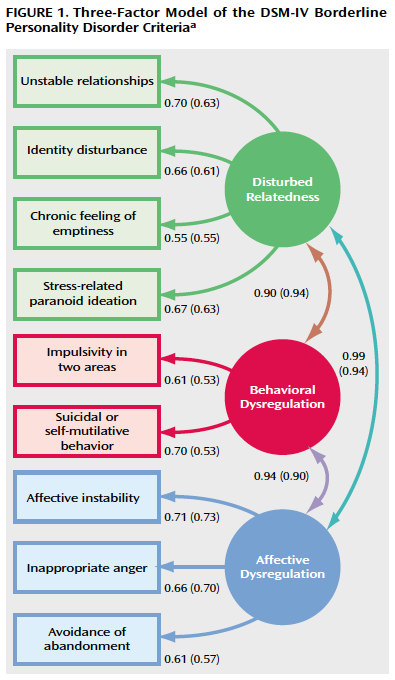
\includegraphics[width=2.75000in,height=4.19332in]{media/image8.png}

\textbf{\emph{TRATTAMENTO CLUSTER B}}

I farmaci non sono curativi, ma aiutano a migliorare la funzionalitá
psichica.

\begin{itemize}
\item
  \textbf{Farmacoterapia}: soltanto mirata ai sintomi, quali:
\end{itemize}

\begin{itemize}
\item
  \emph{Impulsività/ disregolazione affettiva}: stabilizzatori, (AD)
\item
  \emph{Discontrollo impulsivo}: SGA, stabilizzatori {[}motrigina é il
  piú indicato; acido valproico; carbamazepina{]}
\item
  \emph{Pensiero quasi psicotico, derealizzazione}: SGA
\end{itemize}

\begin{quote}
Sono più utili nel mitigare i sintomi gli stabilizzatori dell'umore
(farmaco di prima scelta), perché agiscono sull'impulsività ed un po'
meno sull'instabilità affettiva, che ha connotazioni differenti nel
paziente borderline rispetto al paziente con disturbi dell'umore. Non si
usa litio e antidepressivi triciclici, perché hanno un basso indice
terapeutico e perché, se assunti in grandi quantità, possono causare la
morte per overdose: si preferiscono per questo motivo gli
antiepilettici.
\end{quote}

\begin{itemize}
\item
  \textbf{Psicoterapia a lungo termine} (4-5 tipi di psicoterapia che
  funzionano nei pazienti borderline, cioè che riducono i comportamenti
  suicidari ma non riducono gli altri fattori)
\item
  \textbf{Psicoeducazione a paziente e famiglie (}spiegare che né il pz,
  né i familiari sono colpevoli del disturbo, ma sono tutti responsabili
  della cura)
\end{itemize}

\textbf{\emph{CLUSTER C:}}

\begin{itemize}
\item
  \textbf{\emph{DP EVITANTE:}}
\end{itemize}

Inibizione sociale per pervasivi sentimenti di inadeguatezza e timore di
critica o umiliazione. Soggetti timidi in ambito sociale che non escono
spesso perché cronicamente hanno timore in pubblico di provare vergogna.

Evitano i rischi e le attività che implicano un contatto interpersonale

Ritiro e timidezza: difese contro la vergogna (= paura di rivelare
aspetti di sé giudicati inadeguati)

Vergogna e ansia sociale diminuiscono con la famigliarità. Se conoscono
bene le persone, questa paura si calma. I disturbi d'interpersonalità
nel cluster C sono meno gravi che nel cluster B, perché il cluster C
riesce ad avere pochi amici.

\emph{\emph{Anamnesi personale di isolamento sociale e distanza forzata
da luoghi o circostanze; fobie, attacchi di panico. }}

\begin{itemize}
\item
  \textbf{\emph{DP DIPENDENTE:}}
\end{itemize}

Pervasivo bisogno di accudimento che induce ad un comportamento
sottomesso ed adesivo

Paura della separazione per incapacità ad assumersi autonomamente le
responsabilità della propria vita se soli cercano subito un'altra
relazione come fonte di rassicurazione, indipendentemente dalla qualità.
Sono Persone che possono stare anche in relazioni poco appaganti (anche
maltrattati) pur di stare con qualcuno. Spesso le persone che hanno
degli stalker come amanti, sono persone con questo tipo di DP. Il
paranoide è il partner ideale per le persone dipendenti e, raramente,
anche il narcisistico.

Condividono con il borderline la paura della separazione o
l'intolleranza all'abbandono. Tuttavia, nel dp dipendente, la paura
della separazione é strettamente collegata ad un'immagine negativa di
sé. I pz con dp dipendente pensano di non essere in grado di stare da
soli e sono grandiosi nella loro inadeguatezza (non riescono a pagare il
bollo dell'auto da soli, ad andare al lavoro da soli, a vivere in modo
indipendente la propria quotidianitá). Questi pz cercano il prossimo per
rassicurazione e non per bisgono della relazione.

N.B: spesso la dipendenza causa aggressività. Dipendenza= formazione di
compromesso (difende dall'ostilità che contemporaneamente viene
espressa).

\emph{\emph{L'anamnesi personale è di scarsa qualità nelle relazioni
sociali; disturbi depressivi e disturbi dell'adattamento}}

\begin{itemize}
\item
  \textbf{\emph{DP OSSESSIVO-COMPULSIVO:}}
\end{itemize}

Diagnosi differenziale con \emph{disturbo ossessivo--compulsivo o DOC},
caratterizzato dalla presenza di ossessioni e convulsioni che non sono
presenti nel disturbo ossessivo compulsivo della personalità. Non è
chiaro se prima dell'esordio di DOC ci sia sempre una condizione di
disturbo ossessivo-compulsivo della personalità: è presente in un 1/3
dei casi ma non è detto che ci sia, non siamo in presenza infatti di una
relazione di premorbosità.

Pervasive preoccupazione per l'ordine, la perfezione ed il controllo
mentale ed interpersonale (mondo interno).

Eccessiva attenzione ai dettagli e regole, a spese di flessibilità,
larghezza di vedute ed efficienza. Spesso a scapito dei sentimenti e
delle relazioni interpersonali autentiche (mondo esterno).

Eccessiva dedizione alla produttività a spese di attività di svago e
amicizie.

\begin{itemize}
\item
  Controllo di sentimenti propri o altrui (sono persone che nelle
  discussioni devono avere sempre ragione, perché loro sanno cosa è
  giusto o sbagliato)
\item
  Ricerca di perfezione (non del piacere)
\end{itemize}

Miglior funzionamento rispetto agli altri DP (vanno bene a lavoro).
Comorbidità: disturbi di panico, disturbi depressivi, DOC.

\textbf{\emph{TRATTAMENTO CLUSTER C:}}

\begin{itemize}
\item
  SSRI (più BDZ)
\item
  Psicoterapia
\end{itemize}

\begin{itemize}
\item
  DP evitante: cognitivo-comportamentale, psicodinamiche
\item
  DP dipendente e ossessivo compulsivo: psicodinamica
\end{itemize}

\textbf{\emph{ASSOCIAZIONE DI DP: }}

Tra i disturbi di personalità spesso c'è un'altra comorbidità: cioè una
persona non ha solo un disturbo ma ne ha di più. Com`è possibile avere
più DP?

Il DSM V ha fatto un passo in avanti, cambiando modo di classificare.
Oggi diciamo che il paziente ha un disturbo di personalità e ne
quantifichiamo il disfunzionamento e vediamo come si manifesta. Per
quantificare il disfunzionamento ci deve essere un danneggiamento
moderato o grave nel funzionamento della personalità e presenza di uno o
più tratti patologici di personalità (inflessibile, pervasivo, stabile
lungo il tempo cioè fin dalla tarda adolescenza o prima età adulta).

\end{document}
